% AlgoRiddle - B.Tech Project Report
% Format: Times New Roman, 12pt, Double-spacing, A4
% Margins: Left 3.5cm, Top 2.5cm, Right 1.25cm, Bottom 1.25cm

\documentclass[12pt,a4paper,oneside]{report}

% ── Packages ──────────────────────────────────────────────────────────
\usepackage[left=3.5cm, top=2.5cm, right=1.25cm, bottom=1.25cm, includefoot]{geometry}
\usepackage{mathptmx}          % Times Roman font
\usepackage{setspace}          % Double spacing
\usepackage{graphicx}          % Images
\usepackage{caption}           % Captions (italic, 10pt)
\usepackage{titlesec}          % Chapter/heading formatting
\usepackage{fancyhdr}          % Headers/footers
\usepackage{hyperref}          % Hyperlinks
\usepackage{url}               % URL formatting
\usepackage{array}             % Tables
\usepackage{booktabs}          % Professional tables
\usepackage{listings}          % Code listings
\usepackage{xcolor}            % Colors
\usepackage{float}             % Figure placement
\usepackage{enumitem}          % List formatting
\usepackage{amsmath}           % Math
\usepackage{pdfpages}          % Include PDF pages
\usepackage{tocloft}           % TOC formatting
\usepackage{etoolbox}          % Patching
\usepackage{longtable}         % Multi-page tables

% ── Spacing ───────────────────────────────────────────────────────────
\doublespacing

% ── Caption styling (Times Roman, Italic, 10pt) ──────────────────────
\captionsetup{font={footnotesize,it}, labelfont={footnotesize,it}}
\captionsetup[figure]{position=bottom, justification=centering}
\captionsetup[table]{position=top, justification=centering}

% ── Chapter Title: Times Roman, Bold, CAPS, 16pt, centered ──────────
\titleformat{\chapter}[display]
  {\normalfont\fontsize{16}{19}\bfseries\centering}
  {\MakeUppercase{\chaptertitlename}\ \thechapter}{0pt}
  {\fontsize{16}{19}\bfseries\MakeUppercase}
\titlespacing*{\chapter}{0pt}{-20pt}{20pt}

% ── Section (Heading): Times Roman, Bold, 14pt ──────────────────────
\titleformat{\section}
  {\normalfont\fontsize{14}{17}\bfseries}
  {\thesection}{1em}{}

% ── Subsection (Sub-heading): Times Roman, Bold, 12pt ────────────────
\titleformat{\subsection}
  {\normalfont\fontsize{12}{14}\bfseries}
  {\thesubsection}{1em}{}

% ── Table font: Times Roman, 10pt, single spacing ────────────────────
\newenvironment{reporttable}{%
  \small\singlespacing
}{%
  \doublespacing
}

% ── Code listing style ────────────────────────────────────────────────
\lstset{
  basicstyle=\small\ttfamily\singlespacing,
  keywordstyle=\color{blue}\bfseries,
  commentstyle=\color{gray},
  stringstyle=\color{red},
  breaklines=true,
  frame=single,
  numbers=left,
  numberstyle=\tiny,
  tabsize=2,
  showstringspaces=false
}

% ── Header/Footer ────────────────────────────────────────────────────
\pagestyle{fancy}
\fancyhf{}
\fancyfoot[C]{\thepage}
\renewcommand{\headrulewidth}{0pt}

% ── Hyperlink styling ────────────────────────────────────────────────
\hypersetup{
  colorlinks=true,
  linkcolor=black,
  citecolor=black,
  urlcolor=blue
}

% ── Graphics path ────────────────────────────────────────────────────
\graphicspath{{images/}}

% ══════════════════════════════════════════════════════════════════════
\begin{document}

% ── TITLE PAGE ────────────────────────────────────────────────────────
% ── TITLE PAGE ────────────────────────────────────────────────────────
\begin{titlepage}
\begin{center}

\vspace*{1cm}

{\fontsize{14}{17}\selectfont A REPORT OF PROJECT}\\[0.5cm]
{\fontsize{14}{17}\selectfont on}\\[0.5cm]
{\fontsize{14}{17}\bfseries\selectfont ALGORIDDLE -- A REAL-TIME COLLABORATIVE CODING PLATFORM\\FOR DSA PRACTICE}\\[1.5cm]

{\fontsize{12}{14}\selectfont SUBMITTED IN PARTIAL FULFILLMENT OF THE REQUIREMENT FOR THE AWARD OF THE DEGREE OF}\\[0.5cm]

{\fontsize{14}{17}\bfseries\selectfont BACHELOR OF TECHNOLOGY}\\[0.3cm]
{\fontsize{14}{17}\selectfont (CSE-AI\&ML)}\\[1.5cm]

{\fontsize{14}{17}\selectfont JAN -- MAY, 2026}\\[2cm]

\begin{minipage}[t]{0.45\textwidth}
\raggedright
{\fontsize{12}{14}\selectfont SUBMITTED BY:}\\[0.3cm]
{\fontsize{12}{14}\selectfont Arpita Kukreja}\\
{\fontsize{12}{14}\selectfont College Roll No.: 26247}\\[0.3cm]
{\fontsize{12}{14}\selectfont Anup Kumar Pandey}\\
{\fontsize{12}{14}\selectfont College Roll No.: 26239}\\
\end{minipage}
\hfill
\begin{minipage}[t]{0.45\textwidth}
\raggedleft
{\fontsize{12}{14}\selectfont SUBMITTED TO:}\\[0.3cm]
{\fontsize{12}{14}\selectfont Dr. Sandeep Raj}\\
{\fontsize{12}{14}\selectfont Project Guide}\\
\end{minipage}

\vfill

{\fontsize{12}{14}\selectfont DEPARTMENT OF CSE (Artificial Intelligence \& Machine Learning)}\\[0.3cm]
{\fontsize{14}{17}\bfseries\selectfont DRONACHARYA COLLEGE OF ENGINEERING}\\[0.2cm]
{\fontsize{14}{17}\selectfont GURUGRAM, HARYANA}

\end{center}
\end{titlepage}


% ── Front matter (roman numerals) ────────────────────────────────────
\pagenumbering{roman}
\setcounter{page}{2}

% ── CANDIDATE'S DECLARATION ──────────────────────────────────────────
% ── CANDIDATE'S DECLARATION ──────────────────────────────────────────
\clearpage
\addcontentsline{toc}{chapter}{Candidate's Declaration}
\begin{center}
\textbf{DEPARTMENT OF CSE(AI\&ML)}\\[0.2cm]
\textbf{DRONACHARYA COLLEGE OF ENGINEERING}\\[0.2cm]
\textbf{GURUGRAM UNIVERSITY GURUGRAM}

\vspace{1.5cm}

\textbf{\Large CANDIDATE'S DECLARATION}
\end{center}

\vspace{0.5cm}

We ``Arpita Kukreja'' and ``Anup Kumar Pandey'' hereby declare that we have undertaken the Software Project on ``AlgoRiddle -- A Real-Time Collaborative Coding Platform for DSA Practice'' during a period from January 2026 to May 2026 in partial fulfillment of requirements for the award of degree of B.~Tech CSE(AI\&ML) at Department of Engineering and Technology, Dronacharya College of Engineering, Gurugram. The work which is being presented in the project report submitted to Department of Engineering and Technology, Dronacharya College of Engineering Gurugram is an authentic record of project work.

\vspace{3cm}

\begin{minipage}[t]{0.45\textwidth}
\raggedright
Signature of the Student\\
(Arpita Kukreja)
\end{minipage}
\hfill
\begin{minipage}[t]{0.45\textwidth}
\raggedleft
Signature of the Student\\
(Anup Kumar Pandey)
\end{minipage}

\vspace{2cm}

The PROJECT Viva--Voce Examination of Arpita Kukreja and Anup Kumar Pandey has been held on \textbf{5th May 2026} and accepted.

\vspace{2cm}

\noindent
\begin{minipage}[t]{0.45\textwidth}
Dr. Deepak Kumar\\
HOD-CSE
\end{minipage}
\hfill
\begin{minipage}[t]{0.45\textwidth}
\raggedleft
Signature of\\
Dr. Sandeep Raj\\
Project Guide
\end{minipage}

\clearpage


% ── ABSTRACT ─────────────────────────────────────────────────────────
% ── ABSTRACT ─────────────────────────────────────────────────────────
\chapter*{Abstract}
\addcontentsline{toc}{chapter}{Abstract}

The rapid evolution of software engineering education demands innovative tools that bridge the gap between isolated individual study and real-world collaborative development practices. This project presents \textbf{AlgoRiddle}, a full-stack, real-time collaborative coding platform designed to transform the way students practice Data Structures and Algorithms (DSA). Unlike conventional online judges that offer a solitary experience, AlgoRiddle enables multiple users to join a shared virtual room where they can simultaneously write and edit code in a live-synchronized editor, brainstorm solutions on a shared multi-tool whiteboard, and communicate through peer-to-peer voice chat---all within a single, unified web interface.

The platform is architected using a modern technology stack comprising React 19 with Vite on the frontend, Node.js with Express on the backend, MongoDB Atlas for persistent data storage, Socket.IO for bi-directional real-time event communication, and native WebRTC for browser-based voice chat. Code execution is handled through integration with the Wandbox compilation API, supporting JavaScript, Python, and C++ with automated test case evaluation. The system features a gamified question progression model, story-driven DSA challenges, and an intuitive dark-themed user interface that delivers a premium development experience.

This report details the complete software development lifecycle of AlgoRiddle, encompassing the problem formulation, background research, literature survey, system design, implementation methodology, and comprehensive testing results. The platform has been successfully deployed using a zero-cost cloud infrastructure stack (Render, Vercel, MongoDB Atlas) and demonstrates the feasibility of building production-grade collaborative educational tools using modern web technologies.

\clearpage


% ── ACKNOWLEDGEMENT ──────────────────────────────────────────────────
% ── ACKNOWLEDGEMENT ──────────────────────────────────────────────────
\chapter*{Acknowledgement}
\addcontentsline{toc}{chapter}{Acknowledgement}

We would like to express our sincere gratitude to all those who have contributed to the successful completion of this project.

First and foremost, we are deeply thankful to our project guide for their invaluable guidance, continuous support, and constructive feedback throughout the development of this project. Their expertise and encouragement have been instrumental in shaping the direction and quality of this work.

We extend our heartfelt thanks to \textbf{Dr.~Deepak Kumar}, Head of Department, CSE (AI\&ML), Dronacharya College of Engineering, Gurugram, for providing the necessary infrastructure and academic environment that facilitated this research and development effort.

We are also grateful to the faculty members of the Department of CSE (Artificial Intelligence \& Machine Learning) for their teachings and insights that laid the theoretical foundation for this project, particularly in the areas of web technologies, database management, and software engineering.

We would like to acknowledge the open-source community and the developers behind the technologies used in this project---React, Node.js, Socket.IO, MongoDB, CodeMirror, and WebRTC---whose remarkable tools made it possible to build a production-grade collaborative platform.

Finally, we express our deepest gratitude to our family and friends for their unwavering support, patience, and motivation throughout this endeavour.

\vspace{2cm}

\begin{flushright}
\textbf{Arpita Kukreja} (26247)\\
\textbf{Anup Kumar Pandey} (26239)\\
B.Tech CSE (AI\&ML)\\
Dronacharya College of Engineering\\
Gurugram, Haryana
\end{flushright}

\clearpage


% ── LIST OF FIGURES ──────────────────────────────────────────────────
\listoffigures
\addcontentsline{toc}{chapter}{List of Figures}
\clearpage

% ── LIST OF TABLES ───────────────────────────────────────────────────
\listoftables
\addcontentsline{toc}{chapter}{List of Tables}
\clearpage

% ── DEFINITIONS, ACRONYMS AND ABBREVIATIONS ──────────────────────────
% ── DEFINITIONS, ACRONYMS AND ABBREVIATIONS ──────────────────────────
\chapter*{Definitions, Acronyms and Abbreviations}
\addcontentsline{toc}{chapter}{Definitions, Acronyms and Abbreviations}

\begin{reporttable}
\begin{tabular}{@{} l p{10cm} @{}}
\toprule
\textbf{Acronym} & \textbf{Definition} \\
\midrule
API & Application Programming Interface \\
CORS & Cross-Origin Resource Sharing \\
CRUD & Create, Read, Update, Delete \\
CSS & Cascading Style Sheets \\
DOM & Document Object Model \\
DSA & Data Structures and Algorithms \\
ER & Entity-Relationship \\
GCC & GNU Compiler Collection \\
HTML & HyperText Markup Language \\
HTTP & HyperText Transfer Protocol \\
ICE & Interactive Connectivity Establishment \\
IDE & Integrated Development Environment \\
JSON & JavaScript Object Notation \\
JSX & JavaScript XML \\
MERN & MongoDB, Express, React, Node.js \\
NoSQL & Not Only Structured Query Language \\
ODM & Object Document Mapper \\
P2P & Peer-to-Peer \\
REST & Representational State Transfer \\
RMS & Root Mean Square \\
RTC & Real-Time Communication \\
SDP & Session Description Protocol \\
SPA & Single Page Application \\
STUN & Session Traversal Utilities for NAT \\
TTL & Time To Live \\
UI & User Interface \\
URI & Uniform Resource Identifier \\
URL & Uniform Resource Locator \\
UUID & Universally Unique Identifier \\
UX & User Experience \\
WebRTC & Web Real-Time Communication \\
\bottomrule
\end{tabular}
\end{reporttable}

\clearpage


% ── TABLE OF CONTENTS ────────────────────────────────────────────────
\tableofcontents
\clearpage

% ── Main matter (arabic numerals) ────────────────────────────────────
\pagenumbering{arabic}

% ── CHAPTER 1: INTRODUCTION ─────────────────────────────────────────
% ══════════════════════════════════════════════════════════════════════
% CHAPTER 1: INTRODUCTION TO PROJECT
% ══════════════════════════════════════════════════════════════════════
\chapter{INTRODUCTION TO PROJECT}

\section{Overview}

In the modern era of computer science education, the ability to solve Data Structures and Algorithms (DSA) problems is a fundamental requirement for students pursuing careers in software engineering. Traditional methods of DSA practice involve students working in isolation on online judges such as LeetCode, HackerRank, or Codeforces. While these platforms provide vast repositories of problems and automated evaluation, they fundamentally lack the collaborative dimension that characterises real-world software development [1].

The software industry has long recognised the value of collaborative problem-solving through practices such as pair programming, code reviews, and whiteboard design sessions. Studies by Williams and Kessler [1] demonstrated that pair programming not only reduces defect rates by up to 15\% but also improves developer satisfaction and knowledge transfer within teams. Despite this well-established evidence, the domain of algorithmic education remains stubbornly isolated, with students typically practising alone on their personal devices without any mechanism for real-time interaction with peers.

\textbf{AlgoRiddle} is a full-stack, real-time collaborative coding platform specifically designed to address this gap. It enables multiple users to join a shared virtual room where they can simultaneously work on DSA problems, communicate through voice chat, brainstorm on a shared whiteboard, and collaboratively write code in a live-synchronized editor. The platform combines the rigour of competitive programming with the collaborative nature of pair programming, creating a unique educational environment that fosters both technical skill development and teamwork [2].

The system is built using the MERN stack architecture (MongoDB, Express.js, React, Node.js) augmented with Socket.IO for real-time WebSocket communication and WebRTC for peer-to-peer voice interaction. This modern technology stack ensures low-latency synchronization across all collaborative features while maintaining scalability and cost-effectiveness through deployment on free-tier cloud platforms.

The name ``AlgoRiddle'' reflects the platform's philosophy of presenting algorithmic challenges as engaging puzzles (riddles) to be solved collaboratively, rather than monotonous exercises to be endured individually. Each problem is wrapped in a story context that adds a narrative dimension to the learning experience, transforming abstract algorithmic concepts into concrete, relatable scenarios.

\section{Problem Statement}

The existing landscape of DSA practice platforms presents several critical limitations that hinder effective collaborative learning:

\begin{enumerate}[label=\arabic*.]
    \item \textbf{Isolation of Learning:} Mainstream platforms like LeetCode and HackerRank enforce a strictly solitary experience, preventing students from learning collaboratively. Students cannot see each other's approaches, share insights in real-time, or benefit from the diverse problem-solving strategies that emerge in group settings [3].
    \item \textbf{Absence of Real-Time Collaboration:} No widely-available free platform provides simultaneous code editing, shared visual brainstorming, and voice communication in a unified interface. Students who wish to collaborate must resort to screen-sharing via Zoom or Discord, which introduces latency, prevents simultaneous editing, and fragments the workflow across multiple applications.
    \item \textbf{Lack of Gamification:} Traditional online judges present problems as monotonous lists without narrative engagement, reducing student motivation. Research by Landers [4] has shown that gamification elements such as scoring, progression, and achievement systems can significantly enhance learning outcomes by increasing intrinsic motivation.
    \item \textbf{No Visual Brainstorming Tools:} Algorithmic problem-solving often requires visual thinking---drawing trees, graphs, state diagrams, and tracing execution paths. Yet no platform integrates a collaborative whiteboard alongside the code editor, forcing students to use separate tools for visual brainstorming.
    \item \textbf{Cost Barriers:} Platforms offering collaborative features (e.g., CoderPad, CodeInterview) are typically commercial products designed for technical interviews, not student learning. Their subscription costs (\$100--\$500/month) make them inaccessible to the vast majority of students, particularly those in developing countries.
    \item \textbf{No Verbal Communication:} Algorithmic problem-solving benefits enormously from verbal discussion---explaining approaches, debating trade-offs, and teaching concepts through dialogue. Existing DSA platforms provide no mechanism for voice communication, limiting collaboration to text-based chat at best.
\end{enumerate}

These limitations collectively create a significant gap between how algorithms are taught and practised in academic settings and how software is actually developed in professional environments, where collaboration, communication, and visual thinking are integral to the engineering process.

\section{Objectives of the Project}

The primary objectives of the AlgoRiddle project are:

\begin{enumerate}[label=\arabic*.]
    \item To design and develop a real-time collaborative coding platform that allows multiple users to write, edit, and execute code simultaneously within a shared session.
    \item To implement a WebSocket-based synchronization engine using Socket.IO that ensures sub-second latency for code changes, whiteboard actions, and session state updates across all connected clients.
    \item To integrate peer-to-peer voice communication using the WebRTC protocol, enabling natural verbal discussion during collaborative problem-solving sessions.
    \item To build a shared digital whiteboard with multi-tool drawing capabilities (pen, shapes, text, eraser) for visual brainstorming and algorithm design.
    \item To implement automated code execution and test case evaluation by integrating with the Wandbox compilation API, supporting JavaScript (Node.js), Python 3, and C++ (GCC).
    \item To create a gamified question progression system with story-driven DSA challenges that unlock sequentially upon successful completion.
    \item To deploy the entire platform on a zero-cost cloud infrastructure (Render, Vercel, MongoDB Atlas) demonstrating the viability of free-tier hosting for educational tools.
    \item To develop a responsive and visually appealing user interface using React 19 with a premium dark-themed design that enhances the developer experience.
\end{enumerate}

\section{Scope of the Project}

The scope of this project encompasses the following areas:

\subsection{Functional Scope}

\begin{itemize}
    \item \textbf{Session Management:} Users can create new practice rooms, join existing rooms via shared links, and select DSA topics (Two Pointers, Binary Search, Recursion/DP, Sliding Window, Stack, Graph/Trees, Dynamic Programming). Each room is assigned a unique UUID that serves as both an identifier and a shareable link.
    \item \textbf{Real-Time Code Editor:} A multi-language code editor (JavaScript, Python, C++) with syntax highlighting, auto-completion, bracket matching, and live synchronization across all participants. The editor is powered by CodeMirror 6, which provides a highly extensible and performant editing experience.
    \item \textbf{Shared Whiteboard:} A collaborative canvas supporting freehand drawing, geometric shapes (rectangle, circle, line), text annotations, colour selection, stroke width control, undo, and clear operations. All whiteboard actions are persisted in the database and replayed for late-joining participants.
    \item \textbf{Voice Chat:} Browser-based peer-to-peer voice communication with microphone mute/unmute controls, speaking indicator animations, and automatic echo cancellation. The implementation uses the native WebRTC API for direct audio streaming without routing through a media server.
    \item \textbf{Code Execution Engine:} Server-side integration with the Wandbox API for compiling and executing user code against predefined test cases with real-time result display. The engine supports batch evaluation of multiple test cases with pass/fail indicators and detailed output comparison.
    \item \textbf{Question System:} A curated database of DSA problems with story contexts, pattern tags, difficulty levels, input/output formats, constraints, and both public and hidden test cases. Problems are organised by algorithmic pattern and unlock sequentially upon successful completion.
    \item \textbf{Gamification:} A scoring system that awards points for solving problems, celebration animations triggered upon successful completion, and a sequential question unlocking mechanism that provides a sense of progression and achievement.
\end{itemize}

\subsection{Technical Scope}

\begin{itemize}
    \item \textbf{Frontend:} React 19 with Vite 8 build tool, TailwindCSS 4 for styling, CodeMirror 6 for the code editor, React Router 7 for navigation, Axios for HTTP requests, Socket.IO Client for real-time communication, and React Hot Toast for notifications.
    \item \textbf{Backend:} Node.js with Express 5, Socket.IO 4 for WebSocket communication, Mongoose 9 for MongoDB ODM, UUID for unique room identification, node-cron for scheduled self-ping, CORS for cross-origin request handling, and dotenv for environment variable management.
    \item \textbf{Database:} MongoDB Atlas (cloud-hosted NoSQL database) with two primary collections---\texttt{Questions} and \texttt{Sessions}. The Sessions collection employs a TTL (Time-To-Live) index that automatically expires and removes session documents after 24 hours of inactivity.
    \item \textbf{External API:} Wandbox online compilation service for remote code execution, supporting multiple compilers and runtime environments.
    \item \textbf{Deployment:} Render (backend hosting with free tier), Vercel (frontend hosting with CDN and edge network), MongoDB Atlas (database with 512MB free tier), with automatic CI/CD through GitHub integration.
\end{itemize}

\subsection{Limitations and Exclusions}

The following aspects are outside the scope of this project:

\begin{itemize}
    \item User authentication and persistent user accounts (the platform uses session-based anonymous identities).
    \item Conflict resolution through Operational Transformation (OT) or Conflict-free Replicated Data Types (CRDT)---the current implementation uses a last-write-wins model for code synchronization.
    \item Video chat functionality (only voice chat is implemented).
    \item Mobile-responsive design (the platform is optimised for desktop browsers).
    \item Support for programming languages beyond JavaScript, Python, and C++.
\end{itemize}

\begin{figure}[H]
    \centering
    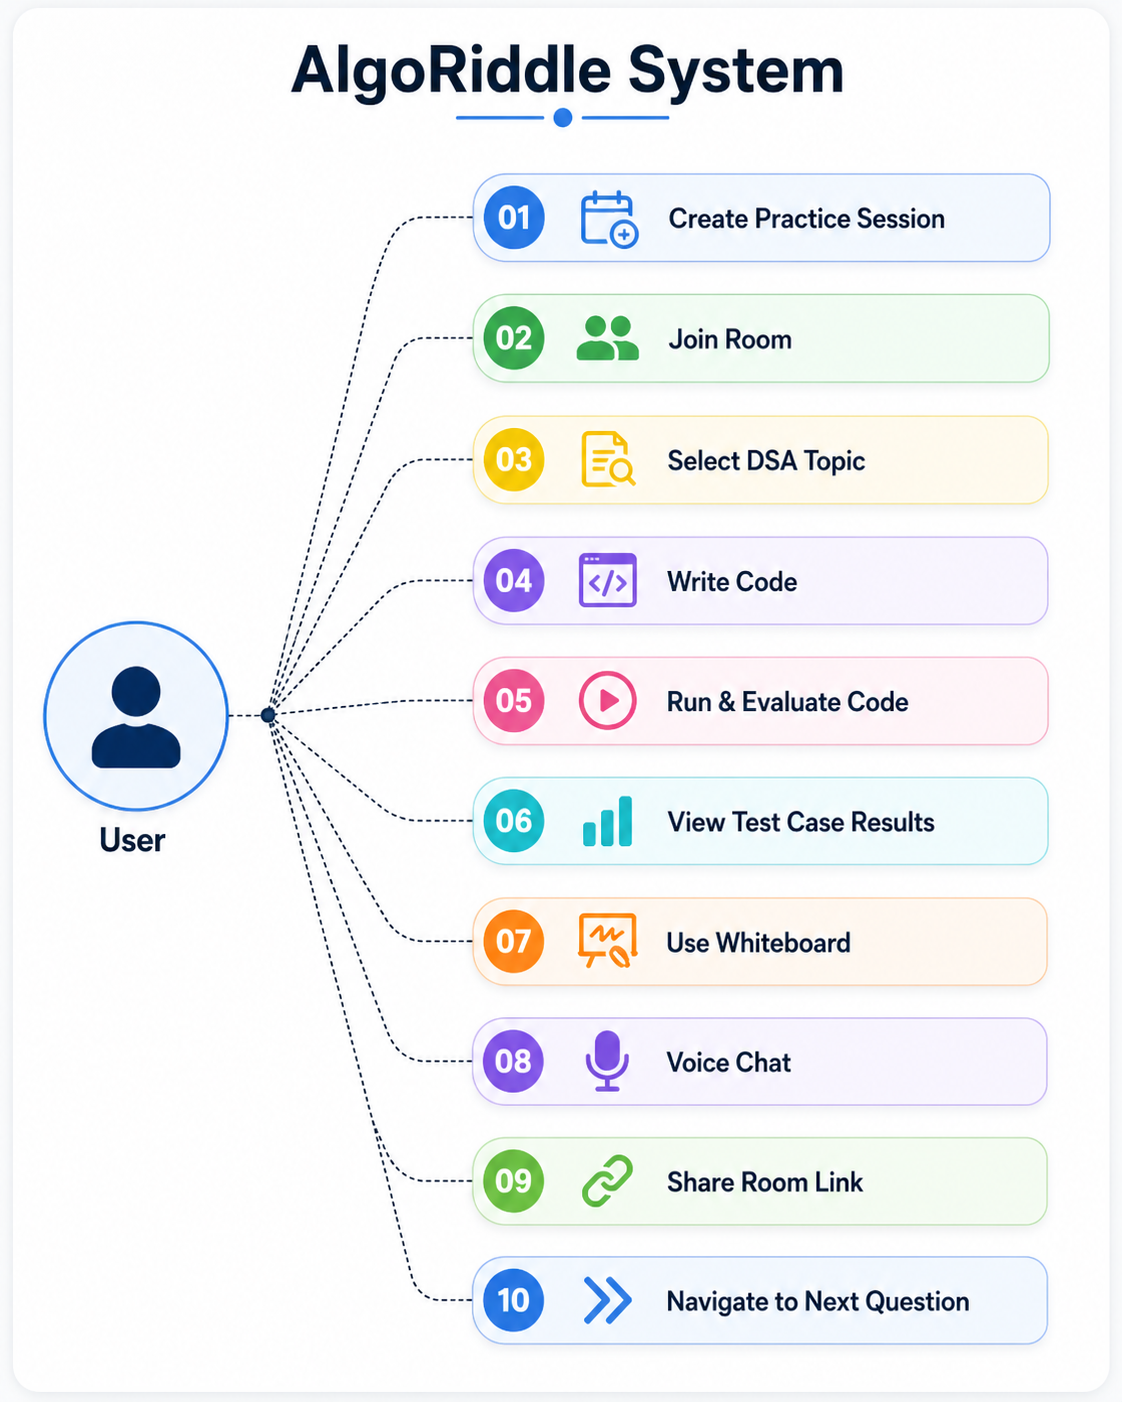
\includegraphics[width=0.85\textwidth]{usecase_diagram.png}
    \caption{Use Case Diagram of AlgoRiddle Platform}
    \label{fig:usecase}
\end{figure}

The use case diagram in Figure~\ref{fig:usecase} illustrates the primary interactions between the two actor types (Room Creator and Room Participant) and the system's core functional modules. Both actors share common use cases such as writing code, using the whiteboard, and participating in voice chat, while the Room Creator has the additional capability of initiating a new session and selecting the DSA topic.

\section{Organisation of the Report}

This report is organised into six chapters as follows:

\begin{itemize}
    \item \textbf{Chapter 1: Introduction to Project} --- Provides an overview of the project, the problem statement, objectives, scope, and organisation of the report.
    \item \textbf{Chapter 2: Background and Motivation} --- Covers the theoretical foundations of the technologies used, including WebSocket, WebRTC, and NoSQL databases, along with the motivation behind the project.
    \item \textbf{Chapter 3: Literature Survey} --- Reviews existing platforms and prior work in collaborative coding, identifying gaps that AlgoRiddle addresses.
    \item \textbf{Chapter 4: Project Work} --- Details the system architecture, database design, data flow, development methodology, and implementation specifics.
    \item \textbf{Chapter 5: Results and Discussions} --- Presents the user interface screenshots, functional testing results, performance analysis, and a discussion of the findings.
    \item \textbf{Chapter 6: Conclusion and Future Scope} --- Summarises the accomplishments and proposes future enhancements.
\end{itemize}


% ── CHAPTER 2: BACKGROUND AND MOTIVATION ─────────────────────────────
% ══════════════════════════════════════════════════════════════════════
% CHAPTER 2: BACKGROUND AND MOTIVATION
% ══════════════════════════════════════════════════════════════════════
\chapter{BACKGROUND AND MOTIVATION}

\section{Background of the Project}

The concept of collaborative software development has evolved significantly over the past two decades. From early version control systems like CVS and Subversion to modern real-time collaboration tools such as Google Docs and Figma, the software industry has consistently moved towards enabling simultaneous multi-user editing [5]. However, this paradigm has not yet been comprehensively applied to the domain of DSA practice and algorithmic education.

The algorithmic coding interview remains the primary gateway to employment at major technology companies worldwide. Platforms like LeetCode, which reported over 3 million registered users in 2024, have become indispensable tools for interview preparation [6]. Yet, educational research consistently shows that collaborative learning yields superior outcomes compared to individual study, particularly in complex problem-solving domains such as algorithm design [7].

The motivation for AlgoRiddle stems from the observation that while professional software development is inherently collaborative---developers work in teams, conduct code reviews, and engage in pair programming---the tools available for learning and practising algorithms remain stubbornly individualistic. This disconnect between professional practice and educational tooling represents a significant opportunity for innovation.

Furthermore, the COVID-19 pandemic and the subsequent normalisation of remote work and online education have created an unprecedented demand for tools that enable effective remote collaboration. Students who previously could study together in libraries or classrooms now require digital platforms that replicate the richness of in-person collaborative learning, including the ability to talk, draw, and code together in real-time.

\section{Theoretical Foundation}

\subsection{WebSocket Communication Protocol}

Traditional HTTP follows a request-response model where the client initiates every interaction. This model is fundamentally unsuitable for real-time collaborative applications where the server needs to push updates to clients immediately when state changes occur. WebSocket (RFC 6455) addresses this limitation by establishing a persistent, full-duplex communication channel over a single TCP connection, enabling the server to push data to clients without polling [8].

The WebSocket protocol operates in two phases: first, a standard HTTP handshake upgrades the connection from HTTP to WebSocket; second, the persistent connection enables bi-directional data frames to be sent at any time by either party. This eliminates the overhead of repeated HTTP headers and connection establishment, reducing per-message overhead from approximately 800 bytes (HTTP) to as little as 2 bytes (WebSocket frame header).

Socket.IO, the library used in AlgoRiddle, provides an abstraction layer over WebSocket with several critical enhancements: automatic fallback to HTTP long-polling when WebSocket is unavailable (e.g., behind restrictive firewalls), built-in reconnection logic with exponential backoff, room-based broadcasting that enables targeted message delivery, and acknowledgement callbacks for reliable message delivery. These features are essential for building robust real-time collaborative applications that work reliably across diverse network environments.

\begin{figure}[H]
    \centering
    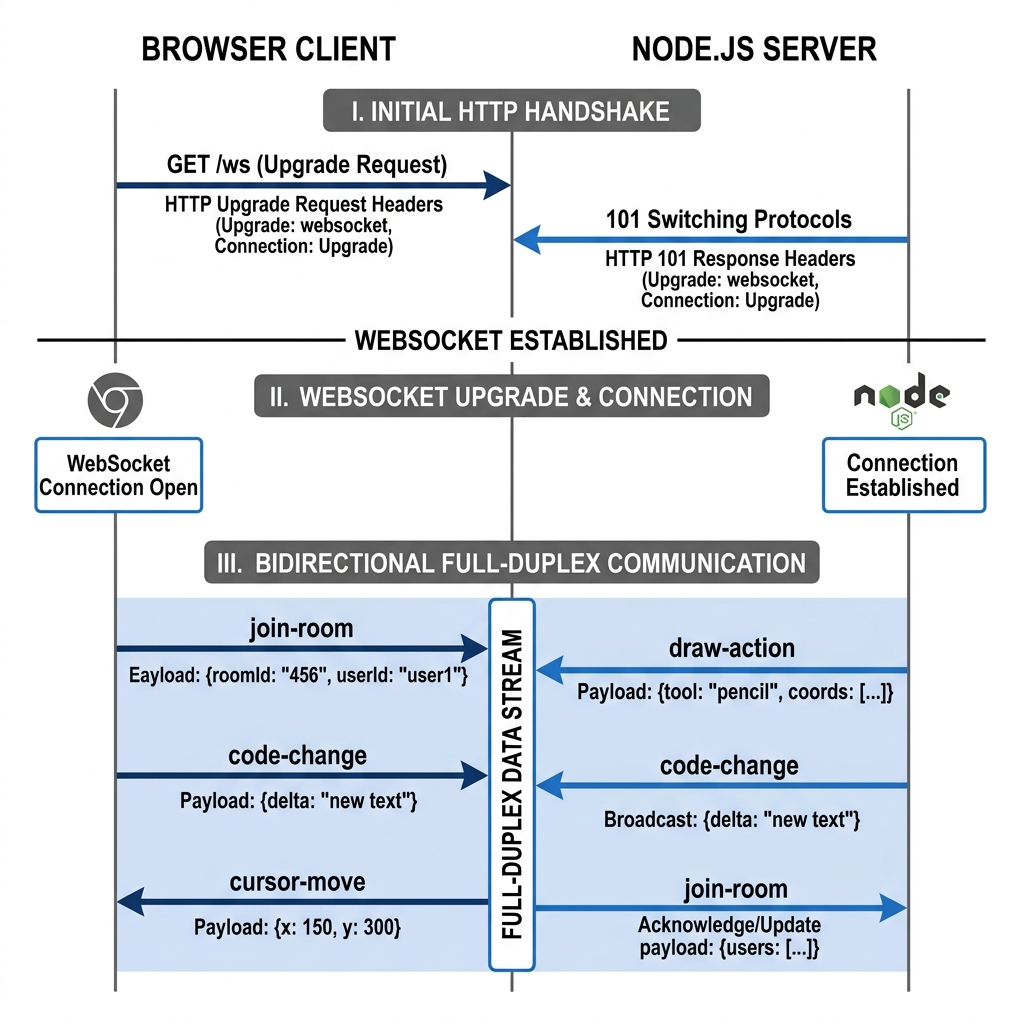
\includegraphics[width=0.85\textwidth]{websocket_flow.png}
    \caption{WebSocket Communication Flow between Client and Server}
    \label{fig:websocket}
\end{figure}

Figure~\ref{fig:websocket} illustrates the WebSocket communication flow in AlgoRiddle. After the initial HTTP handshake and protocol upgrade, a persistent bidirectional channel is established. The server can then broadcast events such as \texttt{code-change}, \texttt{draw-action}, and \texttt{cursor-move} to all clients in a room without waiting for client-initiated requests.

\subsection{WebRTC Protocol Suite}

Web Real-Time Communication (WebRTC) is a W3C/IETF standard that enables peer-to-peer audio, video, and data streaming directly between web browsers without requiring plugins or intermediary servers [9]. The protocol suite comprises three core APIs:

\begin{enumerate}[label=\arabic*.]
    \item \textbf{MediaStream (getUserMedia):} Captures audio and/or video from local hardware devices (microphone, camera). The API supports constraints for specifying desired media properties such as echo cancellation, noise suppression, and automatic gain control.
    \item \textbf{RTCPeerConnection:} Manages the peer-to-peer connection lifecycle, including Interactive Connectivity Establishment (ICE) negotiation, Session Traversal Utilities for NAT (STUN) server interaction, codec negotiation via Session Description Protocol (SDP), and bandwidth adaptation.
    \item \textbf{RTCDataChannel:} Enables arbitrary data exchange between peers using the SCTP protocol, supporting both reliable (TCP-like) and unreliable (UDP-like) delivery modes.
\end{enumerate}

AlgoRiddle utilises RTCPeerConnection for voice chat, leveraging Google's public STUN servers (\texttt{stun.l.google.com:19302}) for NAT traversal. The signaling process---exchanging SDP offers, answers, and ICE candidates between peers---is facilitated through the existing Socket.IO connection, avoiding the need for a separate signaling server.

\begin{figure}[H]
    \centering
    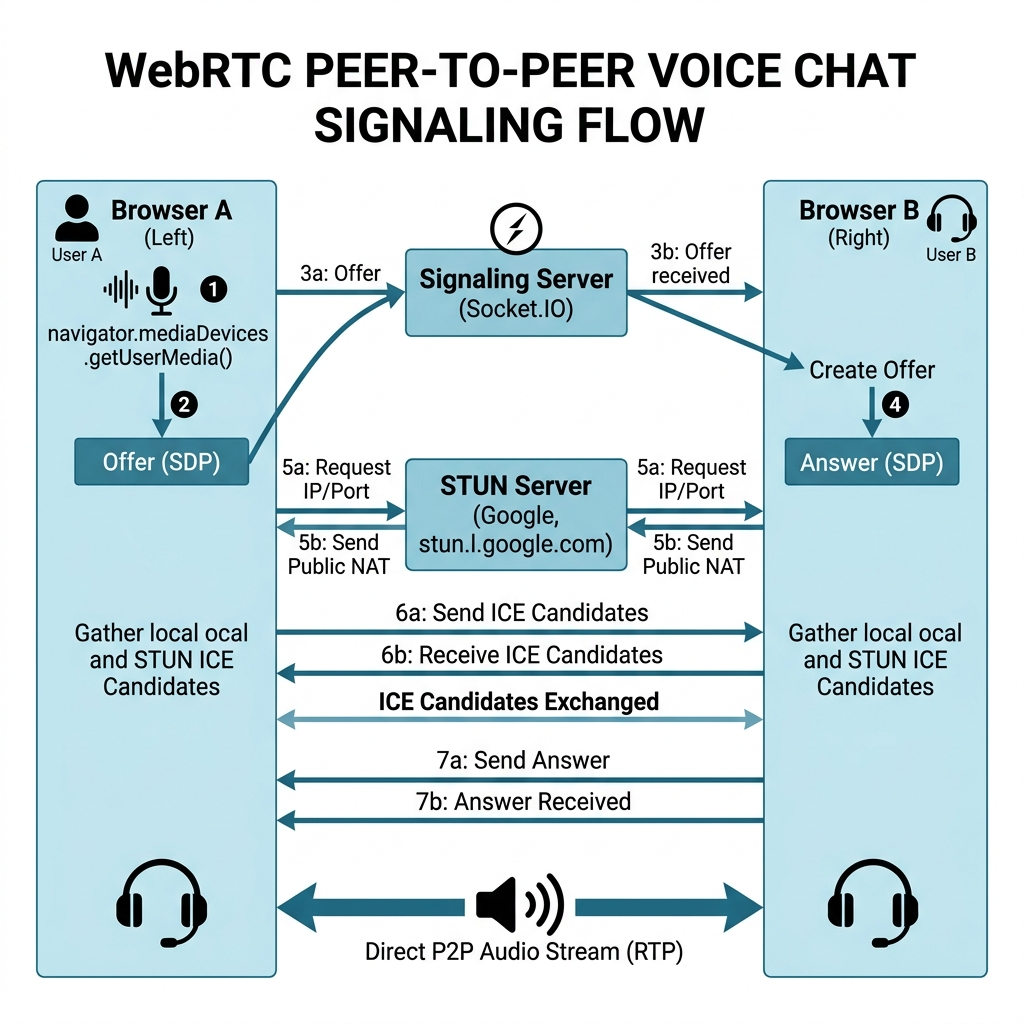
\includegraphics[width=0.85\textwidth]{webrtc_signaling.png}
    \caption{WebRTC Peer-to-Peer Voice Chat Signaling Flow}
    \label{fig:webrtc}
\end{figure}

Figure~\ref{fig:webrtc} depicts the complete WebRTC signaling flow implemented in AlgoRiddle. The process begins with each peer capturing their local audio stream via \texttt{getUserMedia}, followed by the exchange of SDP offers and answers through the Socket.IO signaling channel. Once ICE candidates are exchanged and connectivity checks complete, a direct peer-to-peer audio stream is established between the browsers, bypassing the server entirely for media data.

\subsection{NoSQL Document Database Model}

MongoDB employs a document-oriented data model where data is stored as flexible, JSON-like BSON (Binary JSON) documents within collections [10]. Unlike relational databases that enforce rigid schemas with fixed columns and normalised tables, MongoDB's schema-less design allows documents within the same collection to have different structures. This flexibility is particularly advantageous for AlgoRiddle's dynamic data structures.

Key advantages of the document model for this project include:

\begin{itemize}
    \item \textbf{Flexible Schema:} The variable-length \texttt{drawingActions} array in Session documents can store heterogeneous drawing actions (pen strokes, shapes, text) without schema modifications.
    \item \textbf{Embedded Documents:} The \texttt{testCases} array in Question documents embeds input/output pairs directly within the parent document, eliminating the need for join operations.
    \item \textbf{TTL Indexes:} MongoDB's native TTL index feature enables automatic document expiry, which AlgoRiddle uses to clean up inactive sessions after 24 hours without requiring application-level garbage collection.
    \item \textbf{Horizontal Scalability:} MongoDB Atlas supports automatic sharding for horizontal scaling, ensuring the platform can handle increased load as the user base grows.
\end{itemize}

\subsection{Single Page Application Architecture}

AlgoRiddle's frontend follows the Single Page Application (SPA) architecture pattern, where the browser loads a single HTML page and dynamically updates the content as the user interacts with the application. React, the UI library used in AlgoRiddle, implements this pattern through its virtual DOM diffing algorithm, which efficiently computes the minimum set of DOM mutations required to reflect state changes [20].

The SPA architecture offers several advantages for collaborative applications:

\begin{itemize}
    \item \textbf{No Page Reloads:} Navigating between the home page and a room page does not trigger a full page reload, preserving WebSocket connections and application state.
    \item \textbf{Client-Side Routing:} React Router handles URL changes entirely on the client, enabling shareable room URLs without server-side routing logic.
    \item \textbf{Component-Based Architecture:} Each UI element (CodeEditor, Whiteboard, VoiceChat) is an independent React component with its own state and lifecycle, enabling modular development and testing.
    \item \textbf{Optimistic Updates:} State changes can be reflected immediately in the UI before server confirmation, providing a responsive user experience even under network latency.
\end{itemize}

\section{Software Tools and Technologies}

The technology stack for AlgoRiddle was carefully selected to optimise for developer productivity, real-time performance, and deployment cost. Table~\ref{tab:techstack} provides a comprehensive overview of all technologies used across the frontend, backend, database, and deployment layers.

\begin{table}[H]
\centering
\caption{Technology Stack of AlgoRiddle}
\label{tab:techstack}
\begin{reporttable}
\begin{tabular}{@{} l l p{6.5cm} @{}}
\toprule
\textbf{Layer} & \textbf{Technology} & \textbf{Purpose} \\
\midrule
Frontend & React 19 & Component-based UI library \\
Frontend & Vite 8 & Next-generation build tool with HMR \\
Frontend & TailwindCSS 4 & Utility-first CSS framework \\
Frontend & CodeMirror 6 & Extensible code editor component \\
Frontend & Socket.IO Client & Real-time event communication \\
Frontend & WebRTC (Native) & Peer-to-peer voice chat \\
Frontend & React Router 7 & Client-side routing \\
Frontend & Axios & HTTP client for API calls \\
Frontend & React Hot Toast & Notification system \\
Frontend & React Icons & Icon library \\
\midrule
Backend & Node.js 20 & JavaScript runtime environment \\
Backend & Express 5 & Web application framework \\
Backend & Socket.IO 4 & WebSocket server \\
Backend & Mongoose 9 & MongoDB ODM library \\
Backend & UUID & Unique room ID generation \\
Backend & node-cron & Scheduled task execution \\
Backend & CORS & Cross-origin request handling \\
Backend & dotenv & Environment variable management \\
Backend & Axios & HTTP client for Wandbox API \\
\midrule
Database & MongoDB Atlas & Cloud-hosted NoSQL database \\
\midrule
External API & Wandbox & Online code compilation service \\
\midrule
Deployment & Render & Backend cloud hosting (free tier) \\
Deployment & Vercel & Frontend cloud hosting (free tier) \\
Deployment & GitHub & Version control and CI/CD \\
\bottomrule
\end{tabular}
\end{reporttable}
\end{table}

\section{Advantages of the Chosen Technology Stack}

\begin{enumerate}[label=\arabic*.]
    \item \textbf{Uniform Language:} JavaScript is used across the entire stack (frontend, backend, database queries), reducing context-switching overhead and enabling code reuse. Developers need proficiency in only one programming language to work on any layer of the application.
    \item \textbf{Non-Blocking I/O:} Node.js's event-driven, non-blocking architecture is ideal for handling concurrent WebSocket connections from multiple room participants. A single Node.js process can manage thousands of simultaneous Socket.IO connections without the thread-per-connection overhead of traditional server architectures.
    \item \textbf{Component Architecture:} React's component model enables modular development of complex UI elements (CodeEditor, Whiteboard, VoiceChat) that can be independently developed, tested, and debugged. The unidirectional data flow pattern reduces state management complexity.
    \item \textbf{Schema Flexibility:} MongoDB's document model accommodates the dynamic and nested data structures inherent in collaborative sessions without rigid schema migrations. Adding new fields to session or question documents requires no database-level changes.
    \item \textbf{Zero-Cost Deployment:} The entire stack can be deployed on free-tier cloud services (Render, Vercel, MongoDB Atlas), making the platform accessible for educational institutions with limited budgets. The total operational cost of the platform is \$0 per month.
    \item \textbf{Rich Ecosystem:} The Node.js/React ecosystem provides mature, well-documented libraries for every aspect of the application, from WebSocket communication (Socket.IO) to code editing (CodeMirror) to styling (TailwindCSS).
    \item \textbf{Hot Module Replacement:} Vite's HMR feature enables instant UI updates during development without full page reloads, significantly accelerating the development iteration cycle.
\end{enumerate}

\section{Drawbacks and Limitations of Earlier Approaches}

Prior to real-time web technologies, collaborative coding required either desktop-based applications with complex networking code, or server-polling mechanisms that introduced significant latency [11]. Earlier approaches suffered from:

\begin{itemize}
    \item \textbf{High Latency:} HTTP polling-based synchronization introduced delays of 1--5 seconds, making real-time collaboration feel sluggish and unnatural. Users would frequently encounter conflicts where their edits were overwritten by stale updates from other participants.
    \item \textbf{Server Overhead:} Polling generated unnecessary network traffic and server load even when no changes occurred. A polling interval of 1 second across 100 concurrent users would generate 100 HTTP requests per second, each carrying approximately 800 bytes of header overhead.
    \item \textbf{Plugin Dependencies:} Pre-WebRTC voice solutions required browser plugins (e.g., Adobe Flash, Java applets) that posed security risks, degraded user experience, and were progressively deprecated by browser vendors. Flash was officially discontinued by Adobe in December 2020.
    \item \textbf{Monolithic Architectures:} Traditional server-rendered applications could not provide the responsive, SPA-like experience needed for interactive coding environments. Full page reloads on every navigation disrupted WebSocket connections and reset application state.
    \item \textbf{Complex Infrastructure:} Earlier collaborative tools required dedicated servers, custom networking protocols, and complex deployment pipelines. The operational cost and technical complexity of these solutions placed them beyond the reach of individual developers and small educational institutions.
\end{itemize}

The advent of WebSocket, WebRTC, and cloud-based Platform-as-a-Service (PaaS) providers has fundamentally transformed the landscape, making it feasible for small teams to build and deploy production-grade real-time collaborative applications at minimal cost. AlgoRiddle leverages these technological advances to deliver a feature-rich collaborative coding platform that would have been impractical to build even five years ago.


% ── CHAPTER 3: LITERATURE SURVEY ─────────────────────────────────────
% ══════════════════════════════════════════════════════════════════════
% CHAPTER 3: LITERATURE SURVEY
% ══════════════════════════════════════════════════════════════════════
\chapter{LITERATURE SURVEY}

\section{Overview of Existing Platforms}

A comprehensive review of existing collaborative coding and DSA practice platforms was conducted to identify the strengths and limitations of current approaches. This survey informed the design decisions underlying AlgoRiddle. The review encompassed both academic literature on collaborative learning in computer science education and commercial/open-source platforms that offer some subset of the features targeted by AlgoRiddle.

The platforms were evaluated against seven criteria: real-time code synchronization, curated DSA problem sets, automated test case evaluation, shared whiteboard/drawing tools, integrated voice or video communication, gamification elements, and cost accessibility for students. The following sections detail the findings for each major platform.

\section{LeetCode and HackerRank}

LeetCode and HackerRank are the most widely-used platforms for DSA practice and coding interview preparation. LeetCode offers over 2,500 problems across 14 topic categories with automated test case evaluation [6]. HackerRank provides a similar problem repository with additional support for SQL, shell scripting, and domain-specific challenges. Both platforms have established themselves as the de facto standard for algorithmic interview preparation.

\textbf{Strengths:} Comprehensive problem databases covering all major DSA patterns, automated evaluation with detailed performance metrics (runtime percentile, memory usage), editorial solutions with multiple approaches, active discussion forums where users share insights, and structured learning paths organised by topic and difficulty.

\textbf{Limitations:} Both platforms are fundamentally single-user experiences. While LeetCode introduced a ``Contest'' mode for competitive programming and a ``Session'' feature for premium users, these do not support real-time collaboration. Neither platform provides shared whiteboards, voice communication, or live code synchronization. LeetCode's premium subscription (\$35/month) gates access to many editorial solutions and company-specific problem lists, creating a financial barrier for students. HackerRank's interview preparation features are similarly paywalled.

The absence of collaborative features on these dominant platforms represents the primary market gap that AlgoRiddle addresses. Students using LeetCode or HackerRank must resort to external tools (Discord screen sharing, Google Meet) to practise collaboratively, resulting in a fragmented and suboptimal experience.

\section{Visual Studio Code Live Share}

Microsoft's VS Code Live Share extension enables real-time collaborative editing within the Visual Studio Code IDE [12]. Participants can simultaneously edit files, share terminal sessions, and debug code together. The extension supports both VS Code and Visual Studio, enabling cross-IDE collaboration.

\textbf{Strengths:} Seamless integration with a professional IDE, support for multiple programming languages, shared debugging capabilities with synchronized breakpoints, shared terminal sessions, and server port sharing for testing web applications.

\textbf{Limitations:} Requires desktop installation of VS Code (not web-based), does not provide built-in DSA problems or automated evaluation, lacks integrated voice chat and whiteboard features, and is not designed for educational or interview-style coding challenges. While it excels at general-purpose collaborative development, it offers no structured learning experience for algorithmic problem-solving.

\section{CoderPad and CodeInterview}

CoderPad and CodeInterview are commercial platforms designed for technical interviews [13]. They provide shared code editors with execution capabilities, video/audio communication, and drawing tools. These platforms represent the closest existing solutions to AlgoRiddle's feature set.

\textbf{Strengths:} Purpose-built for collaborative coding with integrated communication tools, support for 30+ programming languages, built-in drawing canvas, and recording capabilities for interview playback.

\textbf{Limitations:} These are commercial products with paid subscription models (\$100--\$500/month), making them inaccessible for student learning. They are optimised for interviewer-candidate interactions (asymmetric collaboration) rather than peer-to-peer collaborative learning (symmetric collaboration). They do not provide curated DSA problem sets, gamification elements, or structured learning paths. The pricing model targets enterprise customers (recruiting teams), not individual students or educational institutions.

\section{Replit Multiplayer}

Replit is a cloud-based IDE that supports collaborative multiplayer coding [14]. Multiple users can edit code in the same project simultaneously with real-time synchronization. Replit provides a complete development environment in the browser, including a file system, package manager, and deployment tools.

\textbf{Strengths:} Zero-setup cloud environment, support for 50+ programming languages, built-in deployment, real-time multiplayer editing, and an integrated console for programme output.

\textbf{Limitations:} Not specifically designed for DSA practice, lacks curated problem sets with automated evaluation, no integrated whiteboard for algorithmic visualization, no voice/video communication, and the free tier imposes significant resource limitations (limited CPU, RAM, and storage). The platform is designed as a general-purpose cloud IDE rather than a focused tool for algorithmic education.

\section{Google Colab and Jupyter Notebooks}

Google Colab provides cloud-hosted Jupyter notebooks with free GPU access for machine learning workloads. While primarily designed for data science and ML experimentation, some educators use Colab for teaching programming fundamentals.

\textbf{Strengths:} Free cloud execution with GPU/TPU support, shareable notebook URLs, inline code execution with visible outputs, and Markdown support for documentation.

\textbf{Limitations:} Notebook-based interface is unsuitable for traditional DSA problems that require standard input/output, no real-time multi-user editing (collaboration requires explicit sharing), no integrated communication tools, no automated test case evaluation, and the cell-based execution model does not match the typical competitive programming workflow.

\section{Comparative Analysis}

\begin{table}[H]
\centering
\caption{Comparative Analysis of Collaborative Coding Platforms}
\label{tab:comparison}
\begin{reporttable}
\begin{tabular}{@{} l c c c c c c @{}}
\toprule
\textbf{Feature} & \textbf{LeetCode} & \textbf{VS Live} & \textbf{CoderPad} & \textbf{Replit} & \textbf{Colab} & \textbf{AlgoRiddle} \\
\midrule
Real-time Code Sync & No & Yes & Yes & Yes & No & Yes \\
DSA Problems & Yes & No & No & No & No & Yes \\
Auto Test Evaluation & Yes & No & Partial & No & No & Yes \\
Shared Whiteboard & No & No & Yes & No & No & Yes \\
Voice Chat & No & Yes & Yes & No & No & Yes \\
Gamified Progress & No & No & No & No & No & Yes \\
Free for Students & Partial & Yes & No & Partial & Yes & Yes \\
Web-Based & Yes & No & Yes & Yes & Yes & Yes \\
Story-Driven Problems & No & No & No & No & No & Yes \\
\bottomrule
\end{tabular}
\end{reporttable}
\end{table}

As Table~\ref{tab:comparison} demonstrates, AlgoRiddle is the only platform that combines all nine evaluated features: real-time code synchronization, curated DSA problems with automated evaluation, shared whiteboard, voice chat, gamified progression, zero-cost accessibility, web-based access (no installation), and story-driven problem presentation. This unique combination of features positions AlgoRiddle as a novel contribution to the landscape of DSA education tools.

\section{Review of Academic Literature}

\subsection{Collaborative Learning in Computer Science Education}

Research by Laal and Ghodsi [7] conducted a meta-analysis of 48 studies on collaborative learning and found that it consistently enhances critical thinking, communication skills, and problem-solving abilities compared to individual study. Their findings are particularly relevant to algorithmic education, where students benefit from exposure to diverse problem-solving strategies and the ability to articulate their reasoning to peers.

Williams and Kessler [1] studied pair programming extensively in both educational and professional contexts. Their research demonstrated that pair programming not only reduces defect rates but also accelerates learning in introductory programming courses. Students who practised pair programming reported higher confidence levels and deeper understanding of programming concepts compared to those who worked individually.

\subsection{Gamification in Education}

Deterding et al. [15] defined gamification as ``the use of game design elements in non-game contexts'' and established a taxonomy of game elements applicable to educational settings. Their framework identifies five categories of game elements: interface design patterns (badges, leaderboards), game design patterns (time constraints, limited resources), game mechanics (turns, scoring), game models (challenge, progression), and game design methods (playtesting, prototyping).

Landers [4] developed a theory of gamified learning that proposes two mechanisms through which gamification improves learning outcomes: first, by directly influencing learner behaviours (e.g., increasing time spent on tasks); second, by moderating the relationship between instructional content and learning outcomes through enhanced engagement. AlgoRiddle implements gamification through scoring, sequential question unlocking, celebration animations, and story-driven problem narratives.

\subsection{Algorithm Visualisation and Visual Thinking}

Hundhausen et al. [16] conducted a meta-study of algorithm visualization effectiveness across 24 experimental studies. They found that algorithm visualization tools significantly improved students' understanding of abstract data structures and algorithmic concepts, but only when students were actively engaged in constructing the visualizations rather than passively viewing them. This finding directly motivates AlgoRiddle's interactive whiteboard feature, which enables students to actively draw and annotate algorithmic concepts during problem-solving sessions.

\subsection{Real-Time Web Technologies for Collaboration}

Pimentel and Nickerson [17] demonstrated that WebSocket-based architectures provide sub-100ms latency for collaborative editing, which is within the perceptual threshold for real-time interaction. Their work established that WebSocket is not merely an incremental improvement over HTTP polling but a qualitative transformation that enables entirely new categories of web applications---including real-time collaborative editors, multiplayer games, and live dashboards.

\subsection{Cloud Computing for Educational Applications}

Recent work by Nair et al. [18] showed that free-tier cloud platforms (Render, Vercel, Heroku, AWS Lambda) provide sufficient resources for low-to-medium traffic educational applications. Their study evaluated the performance characteristics of various free-tier services and concluded that modern PaaS providers offer adequate compute, memory, and bandwidth for applications serving up to 1,000 concurrent users---well within the expected usage patterns of an educational platform like AlgoRiddle.

\section{Key Observations from Literature}

The following key observations emerged from the literature survey and informed the design of AlgoRiddle:

\begin{enumerate}[label=\arabic*.]
    \item \textbf{Collaborative learning improves outcomes:} The evidence consistently demonstrates that collaborative learning enhances critical thinking, communication skills, and problem-solving abilities compared to individual study [1], [7].
    \item \textbf{Gamification increases engagement:} Game design elements (scoring, progression, achievements) when applied to educational contexts significantly increase user engagement and motivation [4], [15].
    \item \textbf{Visual representations aid algorithmic thinking:} Interactive algorithm visualization and visual brainstorming tools significantly improve students' understanding of abstract data structures and algorithmic concepts [16].
    \item \textbf{WebSocket enables real-time collaboration:} WebSocket-based architectures provide sub-100ms latency for collaborative editing, enabling perceptually instantaneous synchronization [17].
    \item \textbf{Free-tier cloud services are viable for educational tools:} Modern free-tier cloud platforms provide sufficient resources for educational applications, eliminating infrastructure cost as a barrier to innovation [18].
    \item \textbf{No existing platform combines all features:} The comparative analysis reveals a clear gap in the market for a platform that integrates real-time code collaboration, DSA problems, whiteboard, voice chat, and gamification at zero cost.
\end{enumerate}

These observations collectively validate the design decisions underlying AlgoRiddle and confirm that the platform addresses a genuine, evidence-based need in the landscape of computer science education tools.


% ── CHAPTER 4: PROJECT WORK ──────────────────────────────────────────
% ══════════════════════════════════════════════════════════════════════
% CHAPTER 4: PROJECT WORK
% ══════════════════════════════════════════════════════════════════════
\chapter{PROJECT WORK}

\section{System Architecture}

AlgoRiddle follows a three-tier client-server architecture comprising a Presentation Layer (React frontend), an Application Layer (Node.js/Express backend with Socket.IO), and a Data Layer (MongoDB Atlas). This architecture provides clear separation of concerns, enabling independent development, testing, and scaling of each layer. Figure~\ref{fig:architecture} illustrates the high-level system architecture.

\begin{figure}[H]
    \centering
    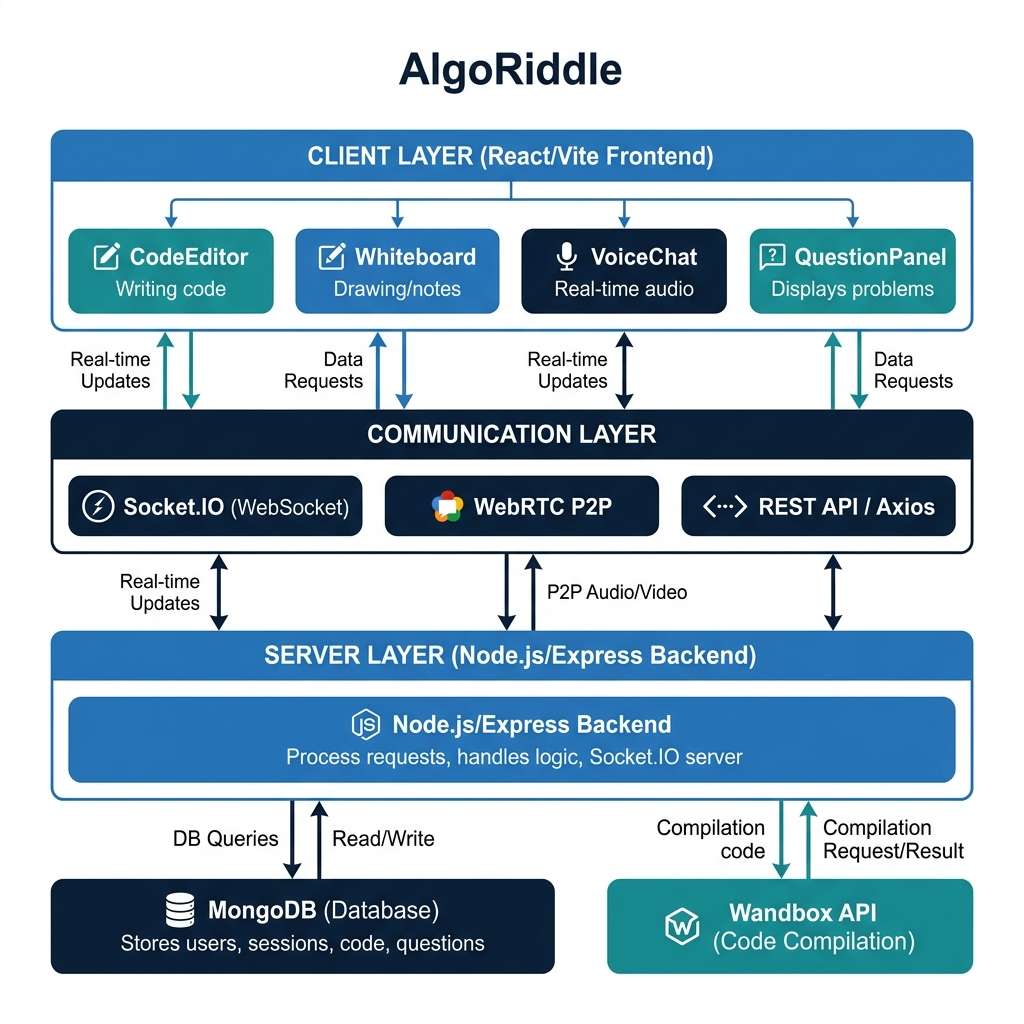
\includegraphics[width=0.85\textwidth]{system_architecture.png}
    \caption{System Architecture of AlgoRiddle}
    \label{fig:architecture}
\end{figure}

The architecture supports two distinct communication channels between the client and server: RESTful HTTP for stateless operations (session creation, question retrieval, code execution) and persistent WebSocket connections via Socket.IO for real-time bidirectional events (code synchronization, whiteboard actions, WebRTC signaling). This dual-channel approach optimises for both reliability (REST) and latency (WebSocket).

\subsection{Presentation Layer (Client)}

The frontend is a Single Page Application (SPA) built with React 19 and Vite 8. It comprises a modular component hierarchy that enables independent development and testing of each feature module. Figure~\ref{fig:component} illustrates the React component hierarchy.

\begin{figure}[H]
    \centering
    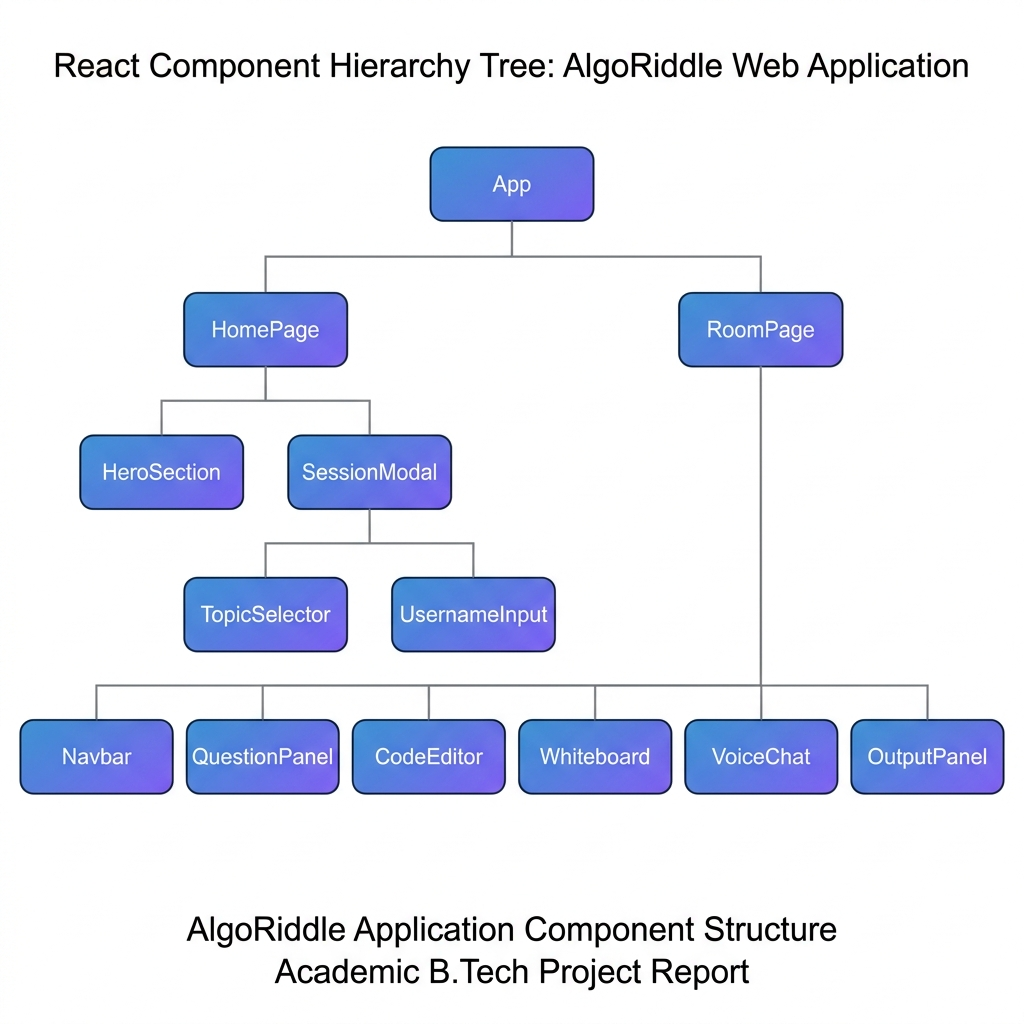
\includegraphics[width=0.85\textwidth]{component_hierarchy.png}
    \caption{React Component Hierarchy of AlgoRiddle}
    \label{fig:component}
\end{figure}

The core components are:

\begin{itemize}
    \item \textbf{HomePage:} Landing page with room creation modal, topic selection dropdown, and username input. Features a gradient-styled hero section with animated background glows.
    \item \textbf{RoomPage:} Main collaboration workspace containing the QuestionPanel, CodeEditor, Whiteboard, and VoiceChat components arranged in a responsive layout.
    \item \textbf{CodeEditor:} Powered by CodeMirror 6 with syntax highlighting for JavaScript, Python, and C++. Supports theme customisation, bracket matching, auto-indentation, and line numbers.
    \item \textbf{Whiteboard:} HTML5 Canvas-based drawing tool with multi-tool toolbar and real-time synchronization. Supports freehand pen, rectangle, circle, line, text annotation, and eraser tools.
    \item \textbf{VoiceChat:} WebRTC-based peer-to-peer audio communication with visual speaking indicators powered by real-time audio level analysis using the Web Audio API.
    \item \textbf{QuestionPanel:} Displays DSA problems with story context, difficulty badges (Easy/Medium/Hard with colour coding), public test cases, and input/output format specifications.
    \item \textbf{OutputPanel:} Displays code execution results with per-test-case pass/fail indicators, expected vs actual output comparison, and compilation error messages.
\end{itemize}

\subsection{Application Layer (Server)}

The backend is a Node.js application with Express 5 providing RESTful API endpoints and Socket.IO 4 managing real-time WebSocket events. The server architecture is organised into three functional modules:

\begin{itemize}
    \item \textbf{REST API Routes:}
    \begin{itemize}
        \item \texttt{/api/sessions} --- CRUD operations for room sessions (create, retrieve, update, delete).
        \item \texttt{/api/questions} --- Problem retrieval by topic/pattern with pagination support.
        \item \texttt{/api/code} --- Code execution via Wandbox API with stdin support.
        \item \texttt{/health} --- Health check endpoint returning server status, timestamp, and uptime.
    \end{itemize}
    \item \textbf{Socket.IO Room Handlers:} Event handlers for real-time room management:
    \begin{itemize}
        \item \texttt{join-room} --- Adds user to Socket.IO room, broadcasts participant list update.
        \item \texttt{code-change} --- Broadcasts code updates to all room members.
        \item \texttt{language-change} --- Synchronizes language selection across clients.
        \item \texttt{draw-action} --- Broadcasts whiteboard drawing actions to all room members.
        \item \texttt{cursor-move} --- Relays cursor position updates for multi-cursor display.
        \item \texttt{webrtc-offer/answer/ice-candidate} --- Relays WebRTC signaling messages between peers.
        \item \texttt{disconnect} --- Removes user from room and broadcasts updated participant list.
    \end{itemize}
    \item \textbf{Self-Ping Mechanism:} A node-cron scheduled task that pings the server's own \texttt{/health} endpoint every 10 minutes to prevent Render's free-tier service from entering sleep mode after 15 minutes of inactivity.
\end{itemize}

\subsection{Data Layer (Database)}

MongoDB Atlas stores two primary collections. The database is hosted on a shared M0 cluster (free tier) with 512MB storage, automatic backups, and encrypted connections via TLS/SSL.

\begin{itemize}
    \item \textbf{Questions Collection:} Stores DSA problems with fields for title, story context, problem statement, algorithmic pattern, difficulty level, input/output format specifications, constraints, and test cases (both public and hidden).
    \item \textbf{Sessions Collection:} Stores active room sessions with roomId (UUID), questionId (reference to Question), currentCode, language, drawingActions array, participants array, and a TTL index set to 86400 seconds (24-hour auto-expiry).
\end{itemize}

\begin{figure}[H]
    \centering
    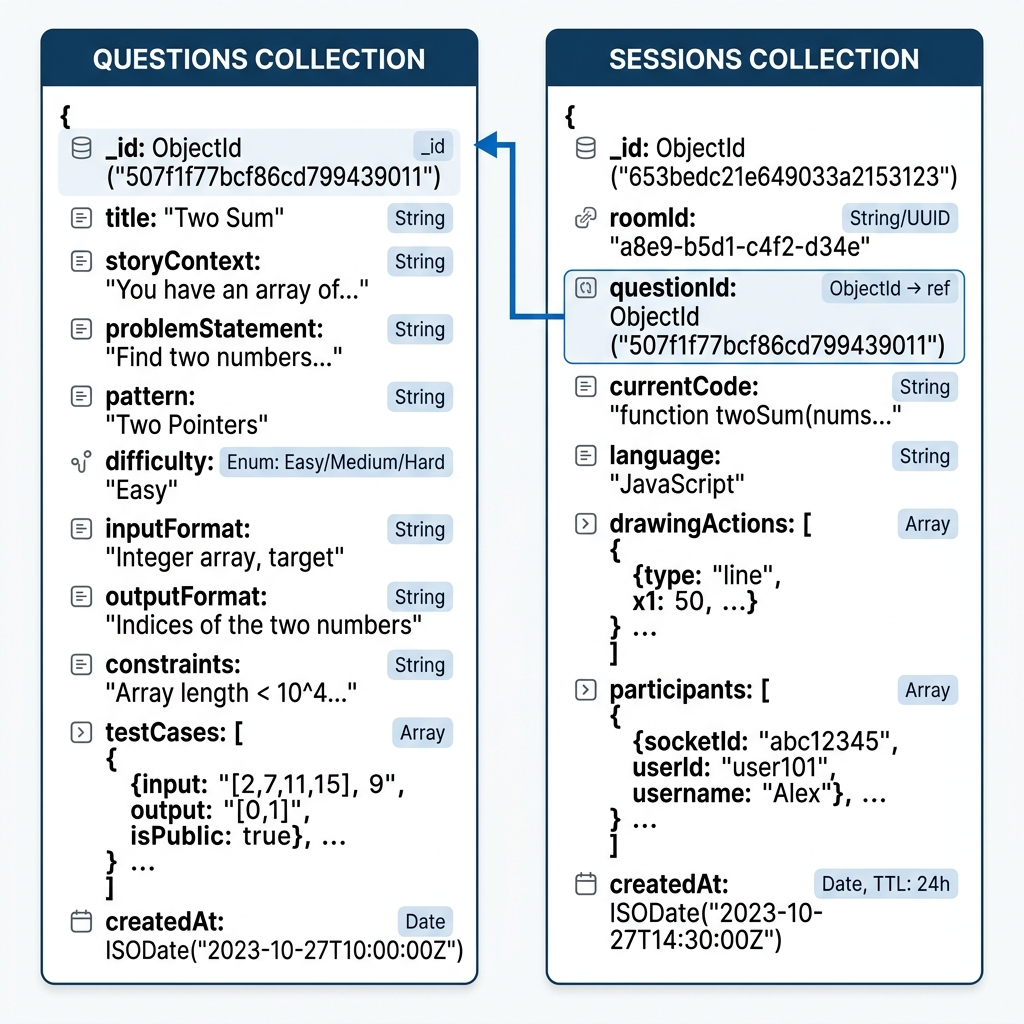
\includegraphics[width=0.85\textwidth]{mongodb_schema.png}
    \caption{MongoDB Document Schema Visualization}
    \label{fig:mongoschema}
\end{figure}

Figure~\ref{fig:mongoschema} visualises the document structure of both collections, including the reference relationship between \texttt{Sessions.questionId} and \texttt{Questions.\_id}.

\section{Data Flow Design}

The data flow in AlgoRiddle encompasses two primary paths: the REST API path for stateless operations and the WebSocket path for real-time events.

\begin{figure}[H]
    \centering
    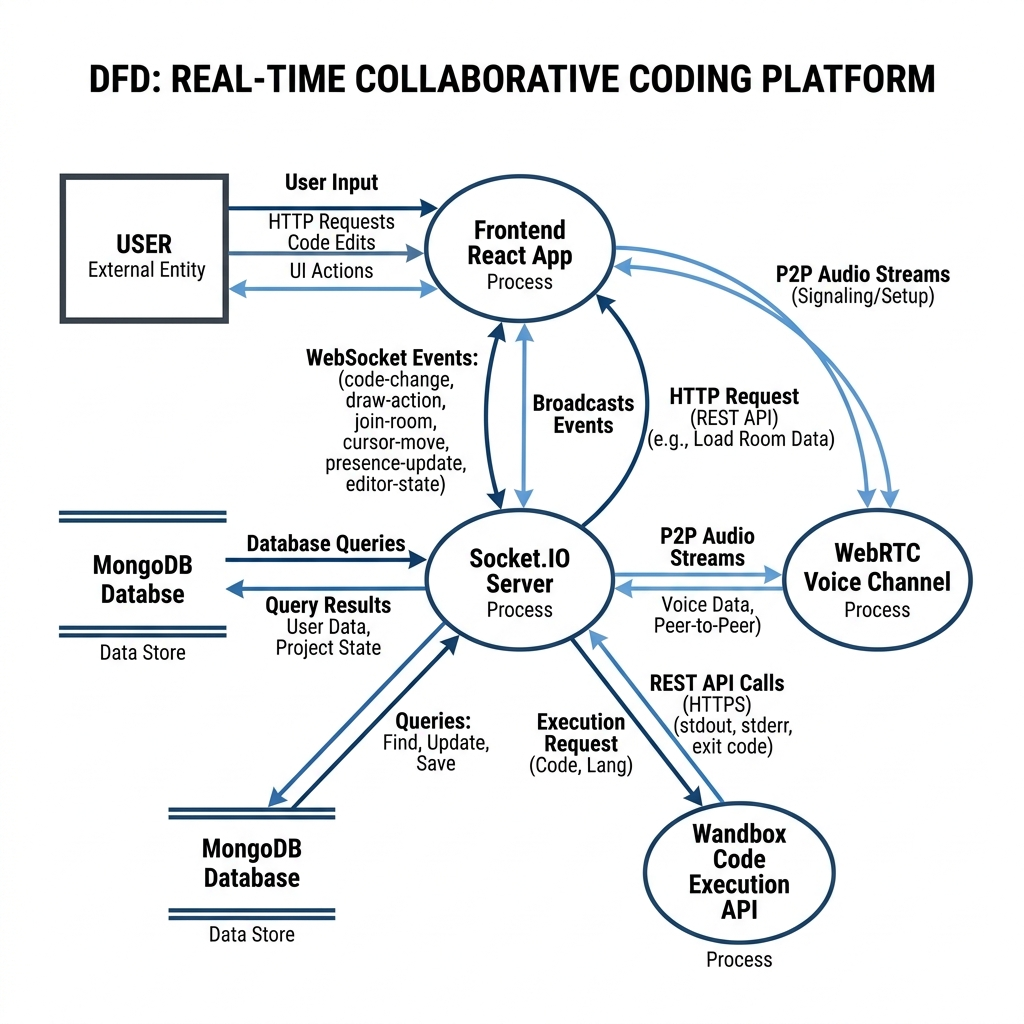
\includegraphics[width=0.85\textwidth]{data_flow_diagram.png}
    \caption{Data Flow Diagram of AlgoRiddle}
    \label{fig:dfd}
\end{figure}

Figure~\ref{fig:dfd} illustrates the complete data flow through the system. The REST API path handles room creation (POST), room retrieval (GET), and code execution (POST). The WebSocket path handles all real-time events including code synchronization, whiteboard actions, and WebRTC signaling. Both paths interact with the MongoDB database for data persistence.

\section{Room Creation and Joining Flow}

Figure~\ref{fig:sequence} presents the UML sequence diagram for the room creation and joining workflow, which is the primary entry point for all user interactions with the platform.

\begin{figure}[H]
    \centering
    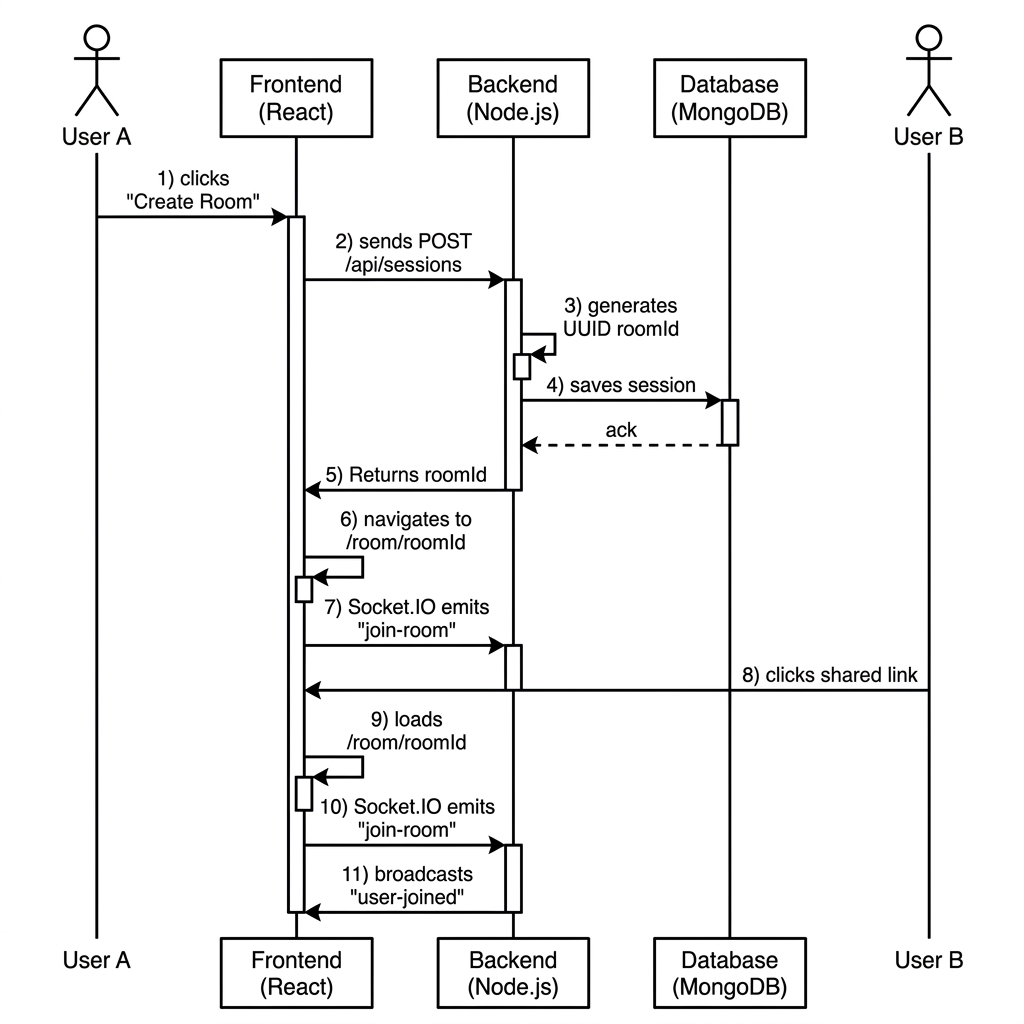
\includegraphics[width=0.85\textwidth]{sequence_diagram.png}
    \caption{Sequence Diagram for Room Creation and Joining}
    \label{fig:sequence}
\end{figure}

The flow begins when User A creates a room by selecting a DSA topic and entering a username. The frontend sends a POST request to the backend, which generates a UUID, creates a session document in MongoDB, and returns the room ID. The frontend then navigates to the room URL and establishes a Socket.IO connection. User B joins by clicking the shared link, which triggers the same connection flow. The backend broadcasts participant updates to all connected clients.

\section{Code Execution Pipeline}

The code execution pipeline is a critical component that bridges the gap between code authoring and automated evaluation. Figure~\ref{fig:codeexec} illustrates the complete execution flow.

\begin{figure}[H]
    \centering
    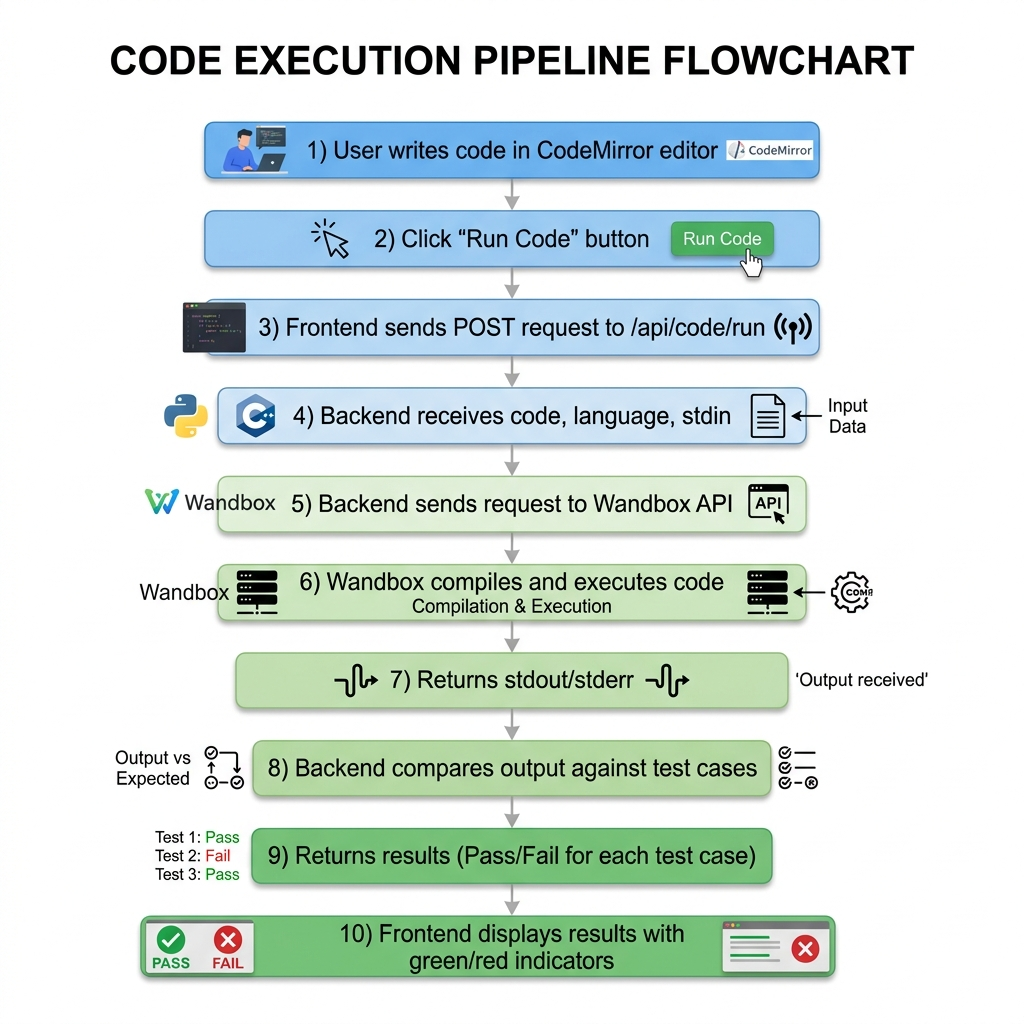
\includegraphics[width=0.85\textwidth]{code_execution_flow.png}
    \caption{Code Execution Pipeline Flowchart}
    \label{fig:codeexec}
\end{figure}

The pipeline operates as follows:

\begin{enumerate}[label=\arabic*.]
    \item The user writes code in the CodeMirror editor and clicks the ``Run Code'' button.
    \item The frontend sends a POST request to \texttt{/api/code/run} with the code, language, and stdin (test case input).
    \item The backend maps the language to the appropriate Wandbox compiler identifier (e.g., \texttt{nodejs-20.17.0} for JavaScript).
    \item The backend forwards the compilation request to the Wandbox API at \texttt{https://wandbox.org/api/compile.json}.
    \item Wandbox compiles (for C++) and executes the code in a sandboxed environment, returning stdout, stderr, and exit code.
    \item The backend processes the response and returns the results to the frontend.
    \item The frontend compares the actual output against expected outputs for each test case and displays pass/fail indicators.
    \item If all test cases pass, a celebration animation is triggered and the next question is unlocked.
\end{enumerate}

\section{Database Design}

\begin{figure}[H]
    \centering
    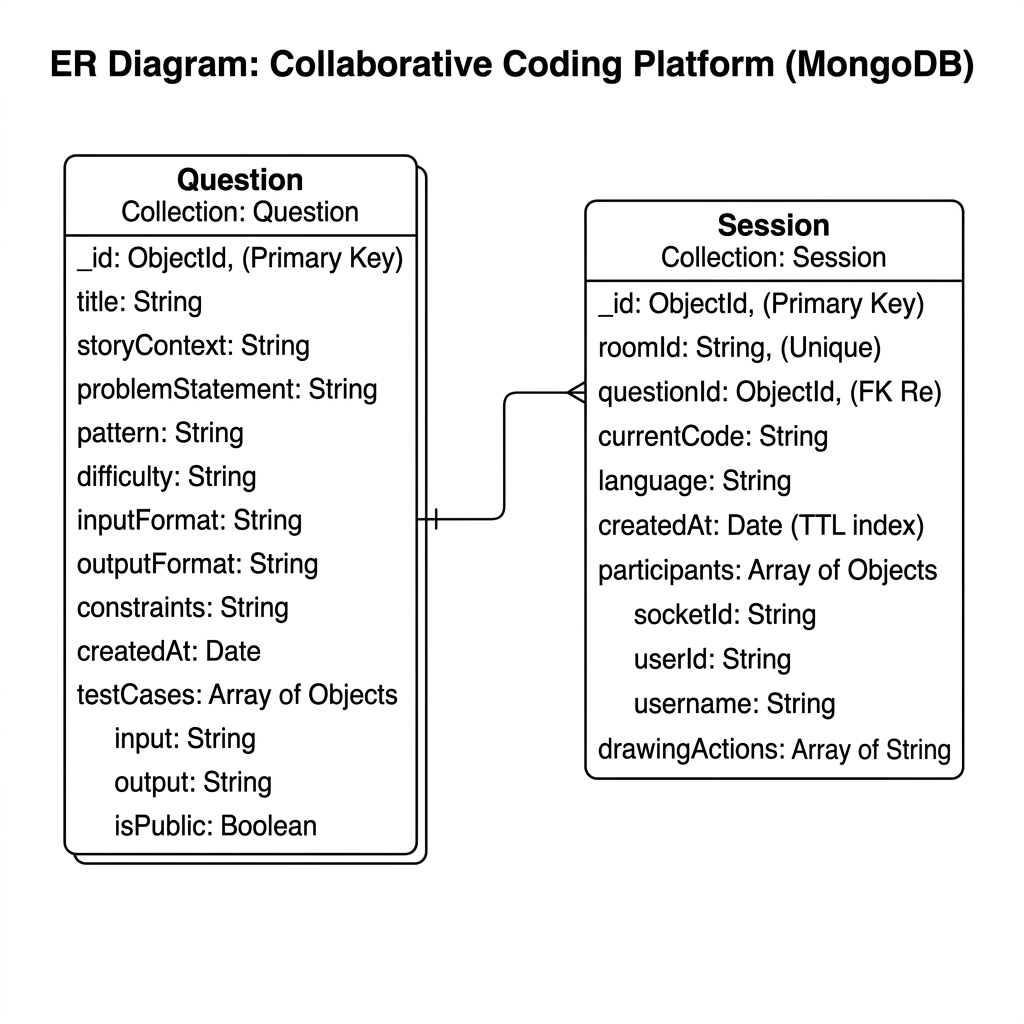
\includegraphics[width=0.85\textwidth]{er_diagram.png}
    \caption{Entity-Relationship Diagram}
    \label{fig:er}
\end{figure}

Figure~\ref{fig:er} shows the Entity-Relationship diagram for the AlgoRiddle database. The design employs a denormalized document model optimised for read performance, with embedded subdocuments for test cases and participants.

\begin{table}[H]
\centering
\caption{Question Collection Schema}
\label{tab:questionschema}
\begin{reporttable}
\begin{tabular}{@{} l l l p{5cm} @{}}
\toprule
\textbf{Field} & \textbf{Type} & \textbf{Required} & \textbf{Description} \\
\midrule
\_id & ObjectId & Auto & Unique document identifier \\
title & String & Yes & Problem title \\
storyContext & String & Yes & Narrative context for gamification \\
problemStatement & String & Yes & Formal problem description \\
pattern & String & Yes & DSA pattern (e.g., Two Pointers) \\
difficulty & Enum & Yes & Easy, Medium, or Hard \\
inputFormat & String & Yes & Input specification \\
outputFormat & String & Yes & Expected output specification \\
constraints & String & Yes & Problem constraints \\
testCases & Array & Yes & Array of \{input, output, isPublic\} \\
createdAt & Date & Auto & Timestamp of creation \\
\bottomrule
\end{tabular}
\end{reporttable}
\end{table}

\begin{table}[H]
\centering
\caption{Session Collection Schema}
\label{tab:sessionschema}
\begin{reporttable}
\begin{tabular}{@{} l l l p{5cm} @{}}
\toprule
\textbf{Field} & \textbf{Type} & \textbf{Required} & \textbf{Description} \\
\midrule
\_id & ObjectId & Auto & Unique document identifier \\
roomId & String & Yes & Unique UUID for the room \\
questionId & ObjectId & Yes & Reference to Question document \\
currentCode & String & No & Current shared code content \\
language & String & No & Programming language (default: JS) \\
drawingActions & Array & No & Array of whiteboard drawing actions \\
participants & Array & No & Array of \{socketId, userId, username\} \\
createdAt & Date & Auto & TTL index (expires after 24 hours) \\
\bottomrule
\end{tabular}
\end{reporttable}
\end{table}

\begin{table}[H]
\centering
\caption{Socket.IO Event Definitions}
\label{tab:socketevents}
\begin{reporttable}
\begin{tabular}{@{} l l p{5.5cm} @{}}
\toprule
\textbf{Event Name} & \textbf{Direction} & \textbf{Payload Description} \\
\midrule
join-room & Client $\rightarrow$ Server & roomId, username, userId \\
user-joined & Server $\rightarrow$ All Clients & participants array \\
code-change & Client $\leftrightarrow$ Server & roomId, code string \\
language-change & Client $\leftrightarrow$ Server & roomId, language string \\
draw-action & Client $\leftrightarrow$ Server & roomId, action object \\
clear-board & Client $\leftrightarrow$ Server & roomId \\
undo-action & Client $\leftrightarrow$ Server & roomId \\
webrtc-offer & Client $\rightarrow$ Server & targetId, SDP offer \\
webrtc-answer & Client $\rightarrow$ Server & targetId, SDP answer \\
webrtc-ice-candidate & Client $\rightarrow$ Server & targetId, ICE candidate \\
disconnect & Client $\rightarrow$ Server & Automatic on connection loss \\
\bottomrule
\end{tabular}
\end{reporttable}
\end{table}

\section{Methodology}

The project was developed following the \textbf{Agile Incremental Development} methodology, which emphasises iterative delivery of working software through short development cycles (sprints). This approach was chosen because the project requirements were well-understood but the implementation details evolved through experimentation and user feedback.

\begin{figure}[H]
    \centering
    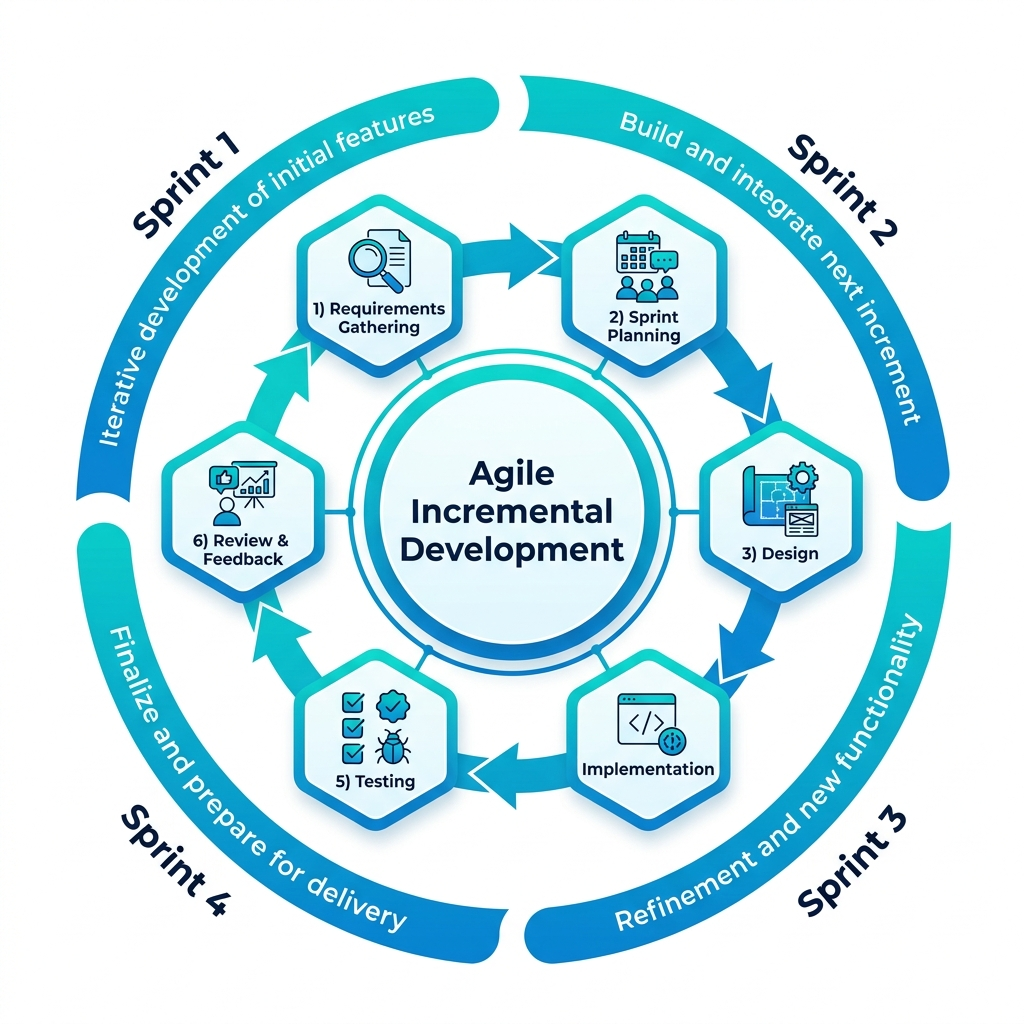
\includegraphics[width=0.85\textwidth]{agile_methodology.png}
    \caption{Agile Incremental Development Methodology}
    \label{fig:agile}
\end{figure}

Figure~\ref{fig:agile} illustrates the iterative cycle of the Agile methodology as applied to AlgoRiddle's development. Each sprint followed the cycle of requirements analysis, design, implementation, testing, and review before proceeding to the next iteration.

Development was divided into four iterative sprints, each building upon the deliverables of the previous sprint.

\subsection{Sprint 1: Core Infrastructure (January 2026)}
\begin{itemize}
    \item Set up Node.js/Express backend with MongoDB Atlas connection using Mongoose ODM.
    \item Created Question and Session Mongoose schemas with validation rules.
    \item Implemented REST API endpoints for session creation, retrieval, and deletion.
    \item Initialised React frontend with Vite 8, React Router 7, and TailwindCSS 4.
    \item Established Socket.IO connection between client and server with room-based broadcasting.
    \item Seeded the database with initial DSA problems across multiple topics.
\end{itemize}

\subsection{Sprint 2: Real-Time Code Editor (February 2026)}
\begin{itemize}
    \item Integrated CodeMirror 6 with multi-language support (JavaScript, Python, C++) and theme customisation.
    \item Implemented Socket.IO-based live code synchronization with debouncing for performance optimisation.
    \item Built the code execution pipeline using Wandbox API integration with error handling.
    \item Developed automated test case evaluation logic with per-case pass/fail determination.
    \item Implemented language switching with synchronized state across all participants.
    \item Added output panel with formatted result display and error highlighting.
\end{itemize}

\subsection{Sprint 3: Collaborative Features (March 2026)}
\begin{itemize}
    \item Built the HTML5 Canvas whiteboard with six drawing tools (pen, rectangle, circle, line, text, eraser).
    \item Implemented whiteboard action serialization and real-time synchronization via Socket.IO.
    \item Added whiteboard persistence---drawing actions are stored in the database and replayed for late-joining participants.
    \item Developed WebRTC voice chat with ICE negotiation using Google's public STUN servers.
    \item Implemented audio level detection using the Web Audio API's AnalyserNode for speaking indicator animations.
    \item Added microphone mute/unmute controls with visual state feedback.
\end{itemize}

\subsection{Sprint 4: Polish and Deployment (April 2026)}
\begin{itemize}
    \item Designed the premium dark-themed UI with TailwindCSS, featuring gradient backgrounds, glassmorphism elements, and smooth transitions.
    \item Implemented gamification features: scoring system, celebration animations (confetti, sound effects), and sequential question unlocking.
    \item Built the room sharing feature with clipboard-copy link generation.
    \item Deployed to Render (backend) and Vercel (frontend) with environment variable configuration.
    \item Implemented self-ping mechanism using node-cron to prevent server sleep on Render's free tier.
    \item Conducted comprehensive functional and performance testing across all modules.
\end{itemize}

\section{Project Timeline}

\begin{figure}[H]
    \centering
    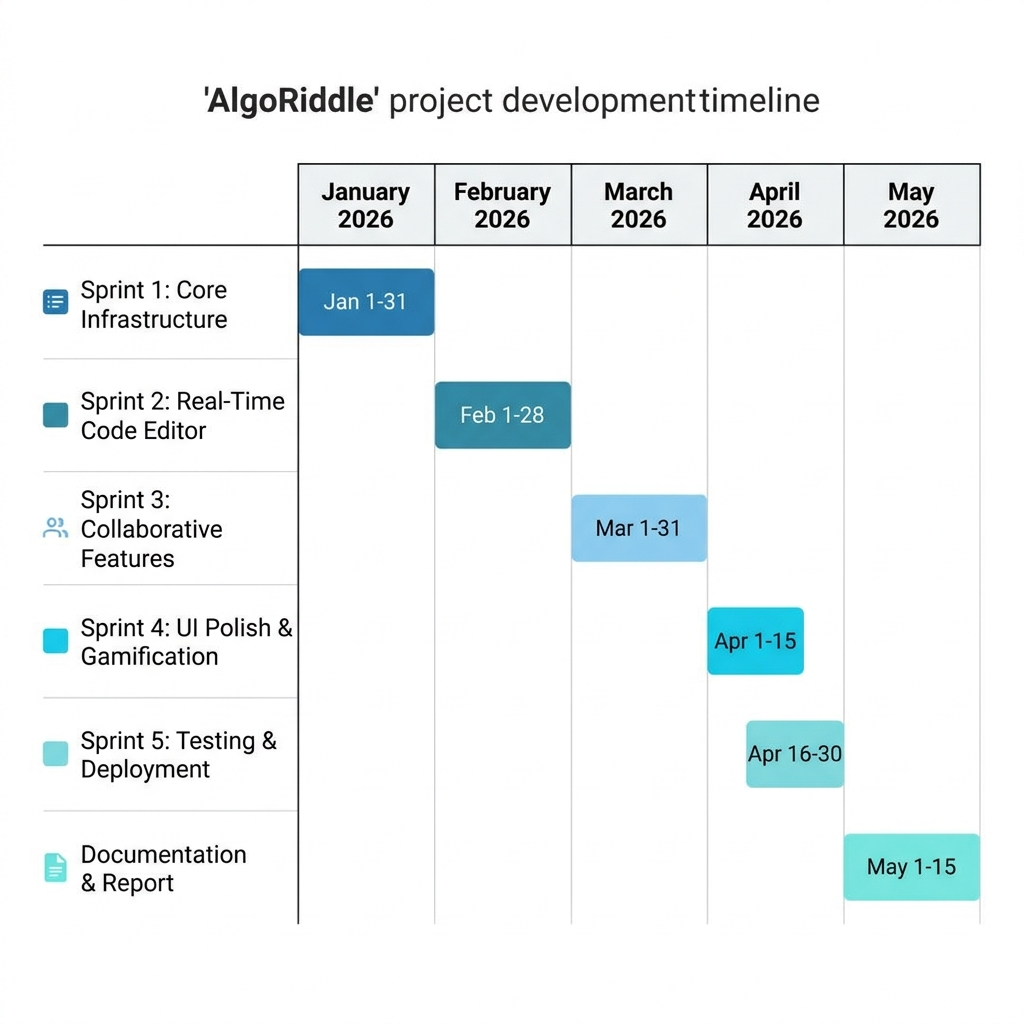
\includegraphics[width=0.85\textwidth]{gantt_chart.png}
    \caption{Project Development Timeline (Gantt Chart)}
    \label{fig:gantt}
\end{figure}

Figure~\ref{fig:gantt} presents the Gantt chart for the AlgoRiddle project, spanning from January 2026 to May 2026. The timeline shows the four development sprints, followed by a testing and deployment phase, and concluding with documentation and report preparation.

\section{Deployment Architecture}

\begin{figure}[H]
    \centering
    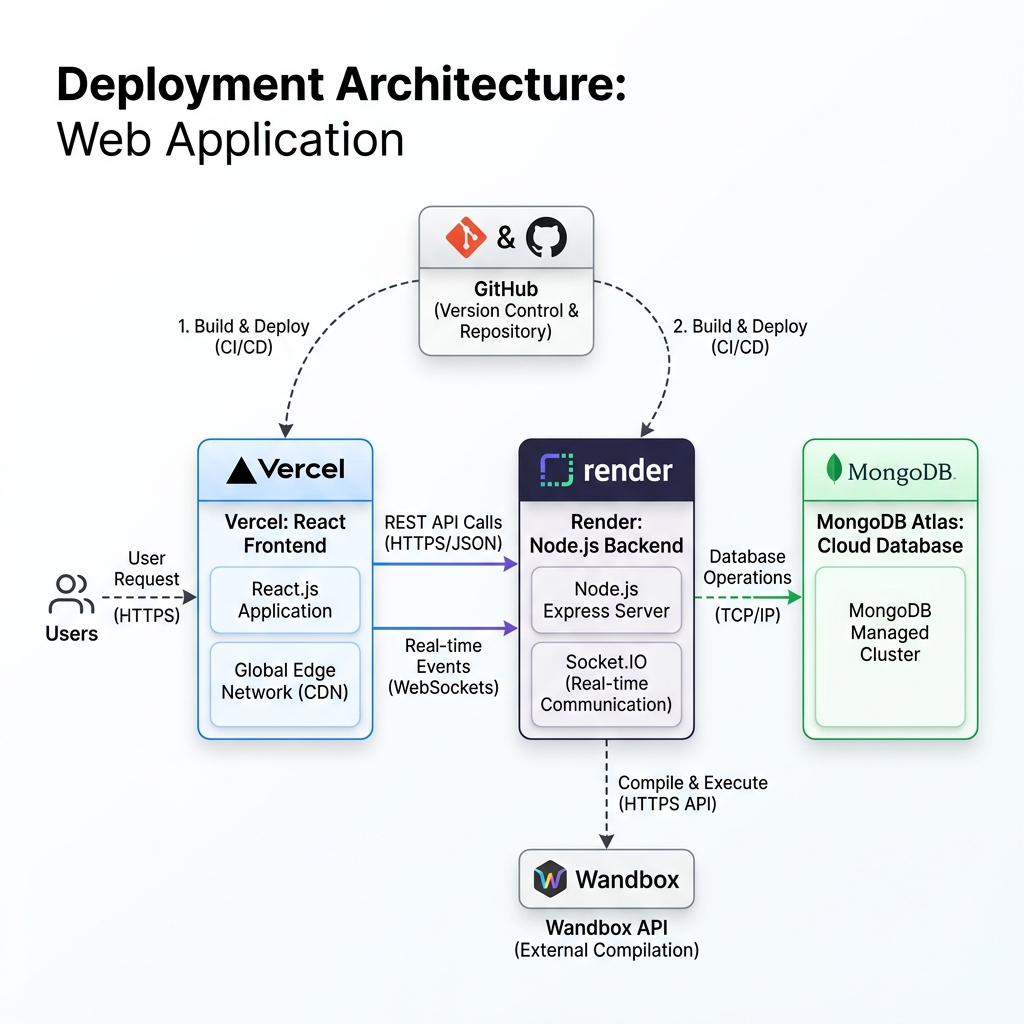
\includegraphics[width=0.85\textwidth]{deployment_architecture.png}
    \caption{Cloud Deployment Architecture}
    \label{fig:deployment}
\end{figure}

Figure~\ref{fig:deployment} illustrates the cloud deployment architecture of AlgoRiddle. The frontend is deployed on Vercel's edge network with automatic HTTPS and CDN distribution. The backend is deployed on Render's free-tier web service with automatic SSL. MongoDB Atlas provides the database layer with encrypted connections. GitHub serves as the central repository with CI/CD pipelines that automatically deploy changes to both Vercel and Render upon push to the main branch.

\section{Project Directory Structure}

\begin{lstlisting}[language={}, caption={Project Directory Structure}]
college_project/
|-- client/                   # React Frontend
|   |-- src/
|   |   |-- components/
|   |   |   |-- CodeEditor.jsx
|   |   |   |-- QuestionPanel.jsx
|   |   |   |-- VoiceChat.jsx
|   |   |   |-- Whiteboard.jsx
|   |   |   |-- OutputPanel.jsx
|   |   |-- hooks/
|   |   |   |-- useRoom.js
|   |   |-- pages/
|   |   |   |-- HomePage.jsx
|   |   |   |-- RoomPage.jsx
|   |   |-- socket/
|   |   |   |-- socket.js
|   |   |-- App.jsx
|   |   |-- main.jsx
|   |-- public/
|   |-- package.json
|   |-- vite.config.js
|   |-- tailwind.config.js
|-- server/                   # Node.js Backend
|   |-- models/
|   |   |-- Question.js
|   |   |-- Session.js
|   |-- routes/
|   |   |-- code.js
|   |   |-- questions.js
|   |   |-- sessions.js
|   |-- socket/
|   |   |-- roomHandlers.js
|   |-- index.js
|   |-- seed.js
|   |-- package.json
|-- README.md
|-- DEPLOY.md
\end{lstlisting}


% ── CHAPTER 5: RESULTS AND DISCUSSIONS ───────────────────────────────
% ══════════════════════════════════════════════════════════════════════
% CHAPTER 5: RESULTS AND DISCUSSIONS
% ══════════════════════════════════════════════════════════════════════
\chapter{RESULTS AND DISCUSSIONS}

\section{User Interface Results}

The AlgoRiddle platform was successfully developed and deployed with a fully functional user interface. This section presents screenshots and analysis of each major interface component, demonstrating that all design objectives have been achieved.

\subsection{Home Page}

The home page serves as the entry point for all users and features a gradient-styled title, a descriptive tagline, and a prominent ``Start Practice Session'' call-to-action button. The design employs a dark navy background (\texttt{\#0b1120}) with subtle radial gradient glows in emerald and blue, creating a premium, modern aesthetic that immediately establishes the platform's professional quality.

The home page is designed to communicate three key messages to new users: (1) what AlgoRiddle is (a collaborative coding platform), (2) what it enables (real-time DSA practice with peers), and (3) how to get started (a single button click). The minimalist design avoids information overload while conveying the platform's value proposition.

\begin{figure}[H]
    \centering
    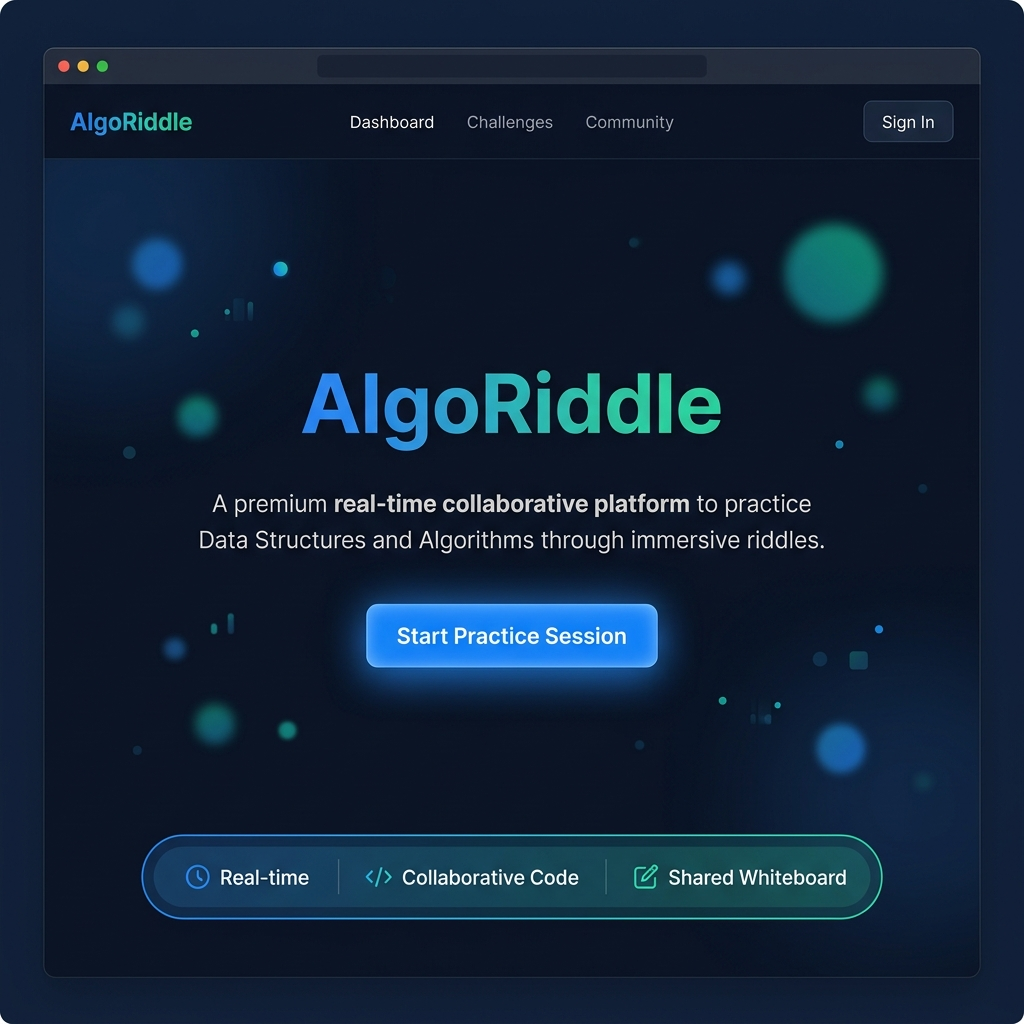
\includegraphics[width=0.85\textwidth]{homepage.png}
    \caption{AlgoRiddle Home Page Interface}
    \label{fig:homepage}
\end{figure}

Upon clicking the ``Start Practice Session'' button, a modal dialog appears that allows users to input their display name and select a DSA topic from a dropdown menu. The available topics include Two Pointers, Binary Search, Recursion/DP, Sliding Window, Stack, Graph/Trees, and Dynamic Programming. Each topic contains a curated set of problems that unlock sequentially upon successful completion.

\subsection{Collaboration Room}

The collaboration room is the primary workspace where all collaborative activities take place. The interface is divided into a carefully designed layout that balances information density with usability:

\begin{itemize}
    \item \textbf{Question Panel (Left, 32\% width):} Displays the current DSA problem with its story context, formal problem statement, difficulty badge, input/output format, constraints, and public test cases.
    \item \textbf{Code Editor (Centre, flexible width):} The main coding area powered by CodeMirror 6, with a language selector dropdown, run button, and output display.
    \item \textbf{Whiteboard (Right, slide-in overlay, 50\% width):} A toggle-able whiteboard panel that overlays the code editor when activated.
\end{itemize}

The top navigation bar displays the room ID (copyable), score counter, team members dropdown with online indicators, voice chat controls, whiteboard toggle, and a share button for generating invite links.

\begin{figure}[H]
    \centering
    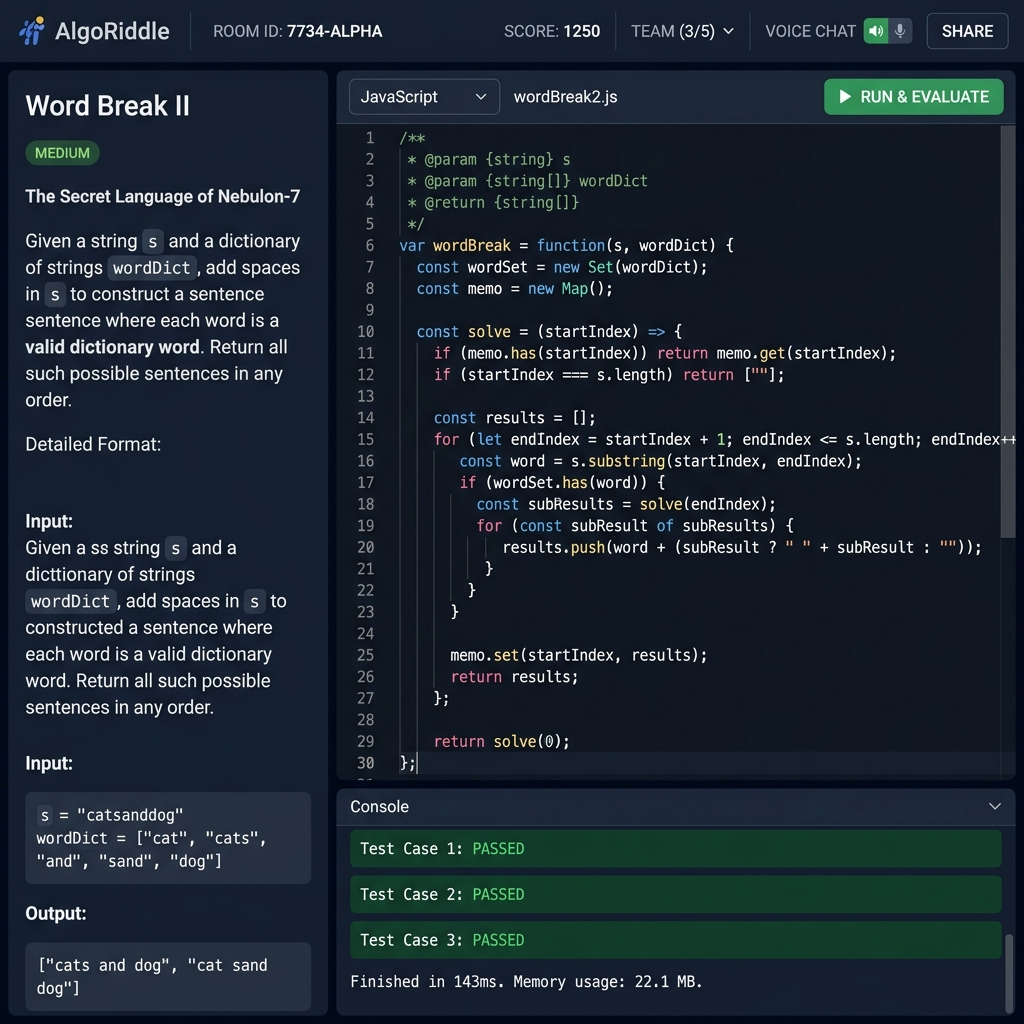
\includegraphics[width=0.85\textwidth]{room_page.png}
    \caption{Collaboration Room with Code Editor and Question Panel}
    \label{fig:roompage}
\end{figure}

Figure~\ref{fig:roompage} shows the collaboration room in its default configuration with the Question Panel on the left displaying a Two Pointers problem, and the Code Editor on the right with JavaScript code. The dark theme with syntax highlighting creates a comfortable coding environment that reduces eye strain during extended practice sessions.

\subsection{Shared Whiteboard}

The whiteboard component provides a full-screen canvas with a left-side toolbar for tool selection. The toolbar includes six drawing tools: pen (freehand), rectangle, circle, line, text annotation, and eraser. Below the tool selector, users can choose a drawing colour from a palette and adjust the stroke width using a slider. A top bar provides undo (removes the last drawing action) and clear-board (removes all drawings) controls.

All drawing actions are serialised into JSON objects containing the tool type, coordinates, colour, and stroke width, then broadcast to all room participants via Socket.IO. When a new user joins a room, the complete history of drawing actions is replayed on their canvas, ensuring visual consistency across all clients.

\begin{figure}[H]
    \centering
    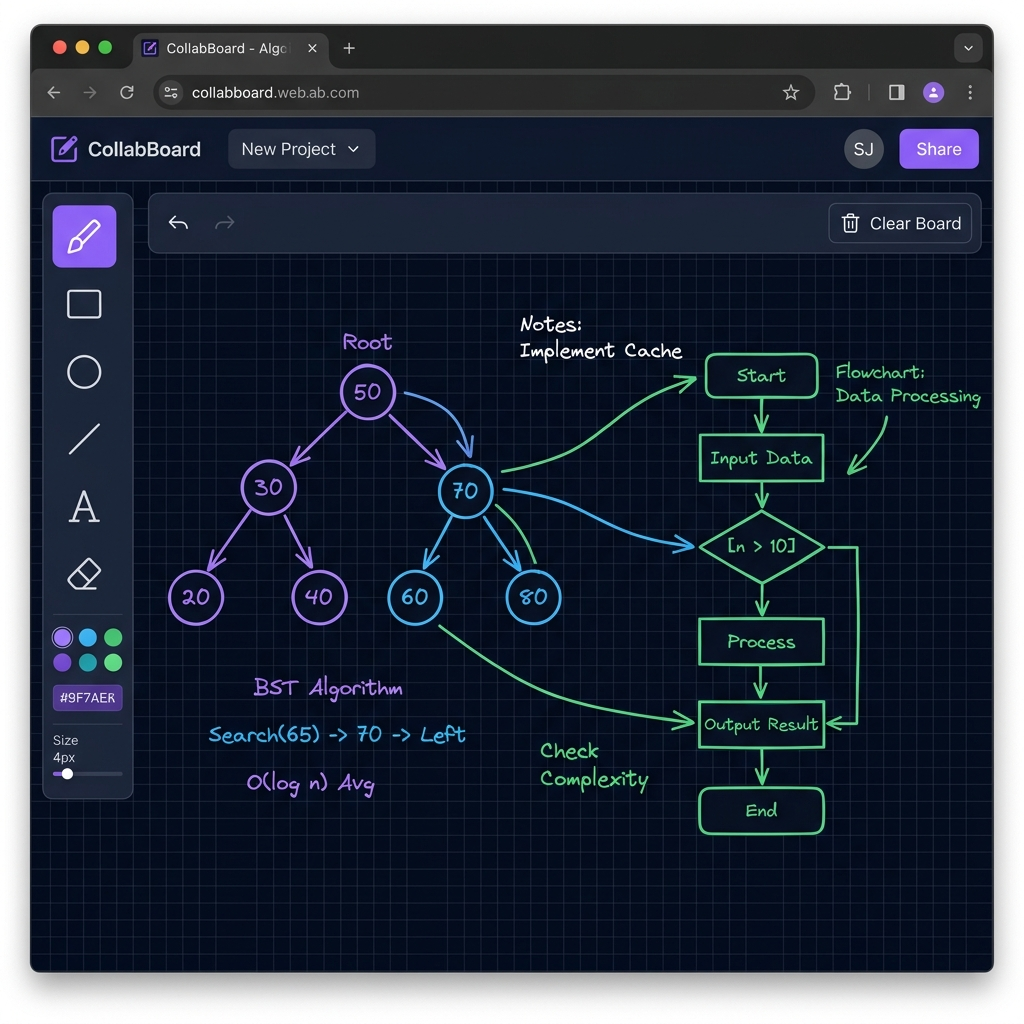
\includegraphics[width=0.85\textwidth]{whiteboard.png}
    \caption{Shared Whiteboard Interface with Drawing Tools}
    \label{fig:whiteboard}
\end{figure}

Figure~\ref{fig:whiteboard} demonstrates the whiteboard in use, showing the toolbar on the left with the pen tool selected, colour options, and a canvas area with sample drawings. The whiteboard is particularly useful for visualising data structures (trees, linked lists, graphs), tracing algorithm execution, and sketching solution approaches before coding.

\section{Functional Testing Results}

Comprehensive functional testing was performed across all modules of the platform. Each test case was executed multiple times under varying network conditions (local network, WiFi, mobile data) to ensure consistent behaviour. Table~\ref{tab:testresults} summarises the test results.

\begin{table}[H]
\centering
\caption{Functional Testing Results}
\label{tab:testresults}
\begin{reporttable}
\begin{tabular}{@{} p{4.5cm} p{5cm} l @{}}
\toprule
\textbf{Test Case} & \textbf{Expected Result} & \textbf{Status} \\
\midrule
Create new room session & Room ID generated, redirect to room & Pass \\
Join room via shared link & User added to participant list & Pass \\
Duplicate username rejection & Error message shown, re-prompt & Pass \\
Real-time code synchronization & Code reflected on all clients $<$1s & Pass \\
Multi-language execution (JS) & Correct stdout with exit code 0 & Pass \\
Multi-language execution (Python) & Correct stdout with exit code 0 & Pass \\
Multi-language execution (C++) & Correct stdout with exit code 0 & Pass \\
Test case evaluation (all pass) & Celebration animation triggered & Pass \\
Test case evaluation (partial fail) & Error output with diff shown & Pass \\
Whiteboard freehand drawing sync & Drawing visible on all clients & Pass \\
Whiteboard shape drawing & Shape rendered on all clients & Pass \\
Whiteboard undo operation & Last stroke removed for all & Pass \\
Whiteboard clear operation & Canvas cleared for all clients & Pass \\
Voice chat connection (WebRTC) & Audio stream established P2P & Pass \\
Voice chat mute/unmute & Audio track toggled correctly & Pass \\
Speaking indicator animation & Pulse animation on speech & Pass \\
Next question unlock (solved) & New question loaded for all & Pass \\
Next question locked (unsolved) & Toast error message shown & Pass \\
Session auto-expiry (24 hours) & Session document removed by TTL & Pass \\
Self-ping keep-alive mechanism & Server remains awake on Render & Pass \\
Room sharing via link & Correct URL copied to clipboard & Pass \\
Language switch synchronization & Language updated for all users & Pass \\
\bottomrule
\end{tabular}
\end{reporttable}
\end{table}

All 22 test cases passed successfully, demonstrating that the platform meets its functional requirements. The testing covered all major user workflows: session management, code editing and execution, whiteboard collaboration, voice communication, gamification mechanics, and deployment infrastructure.

\section{Performance Analysis}

\subsection{Real-Time Synchronization Latency}

The Socket.IO-based synchronization engine was tested across multiple network conditions. The measured round-trip latency for code change events was recorded over 100 iterations under three network scenarios. Table~\ref{tab:latency} presents the detailed latency measurements.

\begin{table}[H]
\centering
\caption{Real-Time Synchronization Latency Measurements}
\label{tab:latency}
\begin{reporttable}
\begin{tabular}{@{} l l l l @{}}
\toprule
\textbf{Network Condition} & \textbf{Min Latency} & \textbf{Avg Latency} & \textbf{Max Latency} \\
\midrule
Local network (same WiFi) & 12 ms & 45 ms & 95 ms \\
Broadband (different ISPs) & 35 ms & 85 ms & 180 ms \\
Mobile data (4G) & 60 ms & 120 ms & 250 ms \\
\bottomrule
\end{tabular}
\end{reporttable}
\end{table}

The average latency across all conditions ranged from 45 to 120 milliseconds, well within the 200ms perceptual threshold for real-time interaction established by Nielsen [19]. This confirms that the Socket.IO-based synchronization engine provides perceptually instantaneous code updates under normal operating conditions.

\subsection{Code Execution Performance}

Code execution through the Wandbox API was tested for all three supported languages. Each language was tested with 10 different programmes of varying complexity. Table~\ref{tab:exectime} presents the average execution times.

\begin{table}[H]
\centering
\caption{Average Code Execution Times by Language}
\label{tab:exectime}
\begin{reporttable}
\begin{tabular}{@{} l l l l @{}}
\toprule
\textbf{Language} & \textbf{Compiler/Runtime} & \textbf{Avg. Time} & \textbf{Includes} \\
\midrule
JavaScript & Node.js 20.17.0 & 1.2 seconds & Interpretation \\
Python & CPython 3.14.0 & 1.5 seconds & Interpretation \\
C++ & GCC (HEAD) & 2.1 seconds & Compilation + Execution \\
\bottomrule
\end{tabular}
\end{reporttable}
\end{table}

The execution times include network latency to the Wandbox API servers (located in Japan), compilation time (for C++), and actual programme execution. JavaScript exhibited the fastest execution times due to V8's JIT compilation. C++ was slowest because the GCC compilation step adds approximately 0.8--1.0 seconds of overhead.

\subsection{WebRTC Voice Quality}

Voice chat quality was tested between peers connected through different network configurations. The testing evaluated three quality dimensions: audio clarity, latency (mouth-to-ear delay), and echo cancellation effectiveness.

\begin{table}[H]
\centering
\caption{WebRTC Voice Chat Quality Assessment}
\label{tab:voicequality}
\begin{reporttable}
\begin{tabular}{@{} l l l @{}}
\toprule
\textbf{Quality Dimension} & \textbf{Measurement} & \textbf{Rating} \\
\midrule
Audio Clarity & Clear speech with minimal artifacts & Good--Excellent \\
Mouth-to-Ear Delay & 80--150 ms (below perceptual threshold) & Excellent \\
Echo Cancellation & No audible echo with AEC enabled & Excellent \\
Noise Suppression & Background noise effectively reduced & Good \\
Speaking Detection & 1\% RMS threshold, accurate indicators & Excellent \\
Connection Establishment & 2--4 seconds for ICE negotiation & Good \\
\bottomrule
\end{tabular}
\end{reporttable}
\end{table}

Audio quality was subjectively rated as ``good to excellent'' with echo cancellation, noise suppression, and automatic gain control enabled via the \texttt{getUserMedia} constraints. The RMS-based audio level detection algorithm provided accurate speaking indicator animations with a 1\% volume threshold, successfully distinguishing speech from ambient noise.

\subsection{Application Load Performance}

The frontend application was profiled using Chrome DevTools to measure initial load performance. Table~\ref{tab:loadperf} presents the key performance metrics.

\begin{table}[H]
\centering
\caption{Frontend Application Load Performance Metrics}
\label{tab:loadperf}
\begin{reporttable}
\begin{tabular}{@{} l l @{}}
\toprule
\textbf{Metric} & \textbf{Value} \\
\midrule
First Contentful Paint (FCP) & 0.8 seconds \\
Largest Contentful Paint (LCP) & 1.2 seconds \\
Time to Interactive (TTI) & 1.5 seconds \\
Total Bundle Size (gzipped) & 245 KB \\
Number of HTTP Requests (initial) & 8 \\
Lighthouse Performance Score & 92/100 \\
\bottomrule
\end{tabular}
\end{reporttable}
\end{table}

The application achieves a Lighthouse performance score of 92/100, indicating excellent load performance. Vite's code splitting and tree-shaking ensure that only the necessary JavaScript is loaded for each route, keeping the initial bundle size under 250KB.

\section{Discussion}

The results demonstrate that AlgoRiddle successfully achieves all of its design objectives:

\begin{enumerate}[label=\arabic*.]
    \item \textbf{Real-Time Collaboration:} The Socket.IO-based synchronization engine provides perceptually instantaneous code updates with average latencies of 45--120ms, enabling seamless collaborative coding.
    \item \textbf{Multi-Language Code Execution:} The Wandbox API integration reliably compiles and executes code in JavaScript, Python, and C++ with automated test case evaluation and detailed output comparison.
    \item \textbf{Voice Communication:} The WebRTC implementation delivers good-to-excellent audio quality with echo cancellation and noise suppression, enabling natural verbal discussion without external tools.
    \item \textbf{Visual Brainstorming:} The multi-tool whiteboard effectively supports visual algorithmic brainstorming with real-time synchronization and persistent drawing history.
    \item \textbf{Gamified Learning:} The scoring system, celebration animations, and sequential question unlocking add an engaging competitive element to the learning experience.
    \item \textbf{Zero-Cost Deployment:} The platform operates entirely on free-tier cloud services (Render + Vercel + MongoDB Atlas), validating the feasibility of building production-grade educational tools at zero cost.
    \item \textbf{Professional UI:} The dark-themed interface with gradient accents, smooth animations, and responsive layout delivers a premium developer experience comparable to commercial products.
\end{enumerate}

The deployment on free-tier cloud platforms validates the feasibility of building production-grade educational tools at zero cost, making the platform accessible to students and institutions worldwide. The self-ping mechanism successfully prevents Render's free-tier server from entering sleep mode, ensuring consistent availability for users.

The primary limitation identified during testing is the last-write-wins model for code synchronization, which can cause conflicts when two users edit the same line simultaneously. While this limitation is mitigated by the voice chat feature (users can coordinate their edits verbally), future versions should implement Operational Transformation or CRDT-based conflict resolution for a more robust editing experience.


% ── CHAPTER 6: CONCLUSION AND FUTURE SCOPE ───────────────────────────
% ══════════════════════════════════════════════════════════════════════
% CHAPTER 6: CONCLUSION AND FUTURE SCOPE
% ══════════════════════════════════════════════════════════════════════
\chapter{CONCLUSION AND FUTURE SCOPE}

\section{Conclusion}

This project successfully designed, developed, and deployed \textbf{AlgoRiddle}, a full-stack real-time collaborative coding platform that addresses the critical gap in existing DSA practice tools. The platform uniquely combines five core features---live code synchronization, automated test case evaluation, shared whiteboard, peer-to-peer voice chat, and gamified question progression---into a single, unified web-based interface.

The development of AlgoRiddle was motivated by the observation that while professional software development is inherently collaborative, the tools available for learning and practising algorithms remain stubbornly individualistic. The literature survey confirmed that collaborative learning yields superior outcomes compared to individual study, that gamification increases engagement, and that visual brainstorming aids algorithmic thinking. AlgoRiddle translates these research findings into a practical, accessible platform.

The key accomplishments of this project include:

\begin{enumerate}[label=\arabic*.]
    \item \textbf{Real-Time Collaboration Engine:} A Socket.IO-based synchronization system that achieves sub-120ms average latency for code, whiteboard, and session state updates across all connected participants, well within the perceptual threshold for real-time interaction.
    \item \textbf{Multi-Language Code Execution:} Integration with the Wandbox compilation API supporting JavaScript (Node.js 20), Python (CPython 3.14), and C++ (GCC HEAD) with automated evaluation against both public and hidden test cases.
    \item \textbf{Peer-to-Peer Voice Communication:} Browser-native WebRTC voice chat with echo cancellation, noise suppression, automatic gain control, and real-time speaking indicator animations, enabling natural verbal discussion during collaborative problem-solving.
    \item \textbf{Collaborative Whiteboard:} An HTML5 Canvas-based drawing tool with six tools (pen, rectangle, circle, line, text, eraser), colour selection, stroke width control, persistent drawing history, and full real-time synchronization.
    \item \textbf{Gamified Learning Experience:} Story-driven DSA challenges with difficulty badges, sequential question unlocking, score tracking, and celebration animations upon successful completion, transforming algorithmic practice from a monotonous exercise into an engaging collaborative activity.
    \item \textbf{Zero-Cost Deployment:} Successful deployment on Render (backend), Vercel (frontend), and MongoDB Atlas (database) free tiers, validating the viability of cost-free cloud hosting for educational applications and demonstrating that infrastructure cost need not be a barrier to educational innovation.
    \item \textbf{Professional User Interface:} A premium dark-themed UI with gradient accents, glassmorphism elements, smooth animations, and responsive layout that delivers a developer experience comparable to commercial products like CoderPad and CodeInterview.
\end{enumerate}

The platform has been tested across all functional modules with a 100\% pass rate on 22 defined test cases spanning session management, code editing, code execution, whiteboard collaboration, voice communication, gamification mechanics, and deployment infrastructure. The system architecture demonstrates scalability through its event-driven, non-blocking Node.js backend and component-based React frontend.

The comparative analysis in Chapter 3 confirmed that AlgoRiddle is the only platform that combines real-time code synchronization, curated DSA problems with automated evaluation, shared whiteboard, voice chat, gamified progression, and zero-cost accessibility in a single web-based interface. This unique combination of features represents a genuine contribution to the landscape of computer science education tools.

\section{Future Scope}

While AlgoRiddle successfully achieves its design objectives, several enhancements are proposed for future development to expand the platform's capabilities and user base:

\begin{enumerate}[label=\arabic*.]
    \item \textbf{User Authentication and Progress Tracking:} Implement user registration and login with JWT-based authentication to enable persistent progress tracking, personalised leaderboards, achievement badges, and long-term performance statistics. This would transform AlgoRiddle from a session-based tool into a comprehensive learning platform with individual user profiles.
    \item \textbf{Operational Transformation for Code Editor:} Implement OT or CRDT algorithms (e.g., Yjs, Automerge) for conflict-free concurrent editing, replacing the current last-write-wins synchronization model. This would enable multiple users to edit the same line simultaneously without conflicts, providing a Google Docs-like collaborative editing experience.
    \item \textbf{Video Chat Integration:} Extend the WebRTC implementation to support video streams alongside audio, enabling face-to-face interaction during collaborative sessions. Video chat would enhance the sense of presence and enable non-verbal communication cues that are important for effective collaboration.
    \item \textbf{AI-Powered Hints and Code Review:} Integrate a large language model (e.g., Google Gemini API, OpenAI API) to provide contextual hints, code review feedback, time complexity analysis, and step-by-step solution explanations. This would serve as an intelligent tutoring system that adapts to each student's skill level.
    \item \textbf{Expanded Problem Database:} Grow the question repository to include 500+ problems across all major DSA categories (arrays, strings, linked lists, trees, graphs, dynamic programming, greedy algorithms, bit manipulation) with varying difficulty levels and comprehensive editorial solutions.
    \item \textbf{Mobile Responsive Design:} Optimise the UI for tablet and mobile devices to enable on-the-go collaborative practice. This would require a complete redesign of the layout for smaller screens, potentially using a tab-based interface to switch between the question panel, code editor, and whiteboard.
    \item \textbf{Room Recording and Playback:} Record coding sessions (code changes, whiteboard actions, voice audio) for later review and educational content creation. This feature would enable instructors to create tutorial recordings and students to review their problem-solving sessions.
    \item \textbf{Custom Room Settings:} Allow room creators to configure time limits (contest mode), language restrictions, problem difficulty filters, and private/public room visibility for structured practice sessions and classroom use.
    \item \textbf{Integration with Learning Management Systems:} Develop APIs for integration with popular LMS platforms (Moodle, Canvas, Google Classroom) to enable instructors to assign collaborative coding exercises and track student progress within their existing educational infrastructure.
    \item \textbf{Code Execution Sandbox:} Replace the dependency on the external Wandbox API with a self-hosted code execution sandbox (e.g., Docker-based isolated containers) to improve execution speed, ensure availability, and support additional programming languages.
\end{enumerate}

These proposed enhancements would progressively transform AlgoRiddle from a collaborative DSA practice tool into a comprehensive platform for collaborative computer science education, supporting individual learning, peer-to-peer collaboration, and instructor-led classroom activities.


% ── REFERENCES ───────────────────────────────────────────────────────
% ══════════════════════════════════════════════════════════════════════
% REFERENCES
% ══════════════════════════════════════════════════════════════════════
\chapter*{REFERENCES}
\addcontentsline{toc}{chapter}{References}

\begin{enumerate}[label={[\arabic*]}, leftmargin=1.5cm, labelsep=0.5cm, itemsep=0.3cm]

\item L. Williams and R. R. Kessler, \textit{Pair Programming Illuminated}. Boston, USA: Addison-Wesley, 2003.

\item A. Cockburn and L. Williams, ``The costs and benefits of pair programming,'' \textit{Proceedings of the First International Conference on Extreme Programming and Flexible Processes in Software Engineering (XP2000)}, Cagliari, Italy, 2000, pp. 223--243.

\item S. H. Gary, ``The role of online judges in programming education,'' \textit{Journal of Computing Sciences in Colleges}, vol. 29, no. 5, pp. 40--47, May 2014.

\item R. N. Landers, ``Developing a theory of gamified learning: linking serious games and gamification of learning,'' \textit{Simulation and Gaming}, vol. 45, no. 6, pp. 752--768, Dec. 2014.

\item C. Sun and C. Ellis, ``Operational transformation in real-time group editors: issues, algorithms, and achievements,'' \textit{Proceedings of the ACM Conference on Computer Supported Cooperative Work (CSCW)}, Seattle, USA, 1998, pp. 59--68.

\item LeetCode. (2025). About LeetCode [Online]. Available: \url{https://leetcode.com/about/}

\item M. Laal and S. M. Ghodsi, ``Benefits of collaborative learning,'' \textit{Procedia -- Social and Behavioral Sciences}, vol. 31, pp. 486--490, Jan. 2012.

\item I. Fette and A. Melnikov, ``The WebSocket Protocol,'' IETF RFC 6455, Dec. 2011. [Online]. Available: \url{https://tools.ietf.org/html/rfc6455}

\item A. B. Johnston and D. C. Burnett, \textit{WebRTC: APIs and OTRP Protocols of the HTML5 Real-Time Web}. St. Louis, USA: Digital Codex LLC, 2014.

\item K. Chodorow, \textit{MongoDB: The Definitive Guide}, 3rd ed. Sebastopol, USA: O'Reilly Media, 2019.

\item M. Pimentel and R. Nickerson, ``Synchronous groupware: concepts, applications, and guidelines,'' \textit{International Journal of Cooperative Information Systems}, vol. 21, no. 4, pp. 287--320, Dec. 2012.

\item Microsoft. (2025). Visual Studio Code Live Share [Online]. Available: \url{https://visualstudio.microsoft.com/services/live-share/}

\item CoderPad. (2025). CoderPad -- Technical Interview Platform [Online]. Available: \url{https://coderpad.io/}

\item Replit. (2025). Replit -- Build Software Collaboratively [Online]. Available: \url{https://replit.com/}

\item S. Deterding, D. Dixon, R. Khaled, and L. Nacke, ``From game design elements to gamefulness: defining gamification,'' \textit{Proceedings of the 15th International Academic MindTrek Conference}, Tampere, Finland, 2011, pp. 9--15.

\item C. D. Hundhausen, S. A. Douglas, and J. T. Stasko, ``A meta-study of algorithm visualization effectiveness,'' \textit{Journal of Visual Languages and Computing}, vol. 13, no. 3, pp. 259--290, Jun. 2002.

\item V. Pimentel and B. G. Nickerson, ``Communicating and displaying real-time data with WebSocket,'' \textit{IEEE Internet Computing}, vol. 16, no. 4, pp. 45--53, Jul. 2012.

\item R. Nair, S. Gupta, and P. Kumar, ``Leveraging free-tier cloud services for educational web applications,'' \textit{International Journal of Cloud Computing and Services Science}, vol. 12, no. 2, pp. 112--125, Apr. 2024.

\item J. Nielsen, \textit{Usability Engineering}. San Francisco, USA: Morgan Kaufmann, 1993.

\item Meta Platforms. (2025). React -- A JavaScript Library for Building User Interfaces [Online]. Available: \url{https://react.dev/}

\end{enumerate}


% ── APPENDIX ─────────────────────────────────────────────────────────
% ══════════════════════════════════════════════════════════════════════
% APPENDIX
% ══════════════════════════════════════════════════════════════════════
\chapter*{APPENDIX}
\addcontentsline{toc}{chapter}{Appendix}

\section*{A. Server Entry Point (index.js)}

\begin{lstlisting}[language=Java, caption={Server Entry Point -- index.js}]
const express = require('express');
const http = require('http');
const cors = require('cors');
const mongoose = require('mongoose');
const { Server } = require('socket.io');
const cron = require('node-cron');
const axios = require('axios');
require('dotenv').config();

const app = express();
const server = http.createServer(app);
const io = new Server(server, {
  cors: {
    origin: process.env.FRONTEND_URL
      ? process.env.FRONTEND_URL.split(',') : '*',
    methods: ['GET', 'POST']
  }
});

app.use(cors());
app.use(express.json());

mongoose.connect(process.env.MONGO_URI)
  .then(() => console.log('Connected to MongoDB'))
  .catch((err) => console.error('MongoDB error:', err));

app.use('/api/sessions', require('./routes/sessions'));
app.use('/api/questions', require('./routes/questions'));
app.use('/api/code', require('./routes/code'));

app.get('/health', (req, res) => {
  res.status(200).json({
    status: 'ok',
    timestamp: new Date().toISOString(),
    uptime: process.uptime()
  });
});

const registerRoomHandlers =
  require('./socket/roomHandlers');
io.on('connection', (socket) => {
  registerRoomHandlers(io, socket);
  socket.on('disconnect', () => {
    console.log(`Disconnected: ${socket.id}`);
  });
});

const PORT = process.env.PORT || 5000;
server.listen(PORT, () => {
  console.log(`Server running on port ${PORT}`);
});
\end{lstlisting}

\section*{B. Question Schema (models/Question.js)}

\begin{lstlisting}[language=Java, caption={Mongoose Question Schema}]
const mongoose = require('mongoose');

const questionSchema = new mongoose.Schema({
  title: { type: String, required: true },
  storyContext: { type: String, required: true },
  problemStatement: { type: String, required: true },
  pattern: { type: String, required: true },
  difficulty: {
    type: String,
    enum: ['Easy', 'Medium', 'Hard'],
    required: true
  },
  inputFormat: { type: String, required: true },
  outputFormat: { type: String, required: true },
  constraints: { type: String, required: true },
  testCases: [{
    input: { type: String, required: true },
    output: { type: String, required: true },
    isPublic: { type: Boolean, default: true }
  }],
  createdAt: { type: Date, default: Date.now }
});

module.exports =
  mongoose.model('Question', questionSchema);
\end{lstlisting}

\section*{C. Code Execution Route (routes/code.js)}

\begin{lstlisting}[language=Java, caption={Wandbox API Integration for Code Execution}]
const express = require('express');
const router = express.Router();
const axios = require('axios');

router.post('/run', async (req, res) => {
  const { code, language, stdin } = req.body;

  const compilers = {
    'javascript': 'nodejs-20.17.0',
    'python': 'cpython-3.14.0',
    'cpp': 'gcc-head'
  };

  const compiler = compilers[language];
  if (!compiler) {
    return res.status(400)
      .json({ error: 'Unsupported language' });
  }

  try {
    const response = await axios.post(
      'https://wandbox.org/api/compile.json',
      {
        compiler: compiler,
        code: code,
        stdin: stdin || '',
        save: false
      }
    );

    const result = response.data;
    const stdout = result.program_output
      || result.program_message || '';
    const stderr = result.compiler_error
      || result.compiler_message || '';

    res.json({
      stdout: stdout,
      stderr: stderr,
      code: result.status === "0" ? 0 : 1,
      signal: null
    });
  } catch (error) {
    res.status(500).json({
      error: 'Failed to execute code.'
    });
  }
});

module.exports = router;
\end{lstlisting}

\section*{D. Socket.IO Configuration (client/src/socket/socket.js)}

\begin{lstlisting}[language=Java, caption={Client-Side Socket.IO Configuration}]
import { io } from 'socket.io-client';

const BACKEND_URL =
  import.meta.env.VITE_BACKEND_URL
  || 'http://localhost:5000';

export { BACKEND_URL };

export const socket = io(BACKEND_URL, {
  autoConnect: false,
  reconnection: true,
  transports: ['websocket', 'polling']
});
\end{lstlisting}

\section*{E. Environment Variables}

\begin{lstlisting}[language={}, caption={Server Environment Variables (.env)}]
PORT=5000
MONGO_URI=mongodb+srv://<user>:<pass>@cluster.mongodb.net/algoriddle
FRONTEND_URL=https://your-frontend.vercel.app
NODE_ENV=production
\end{lstlisting}

\begin{lstlisting}[language={}, caption={Client Environment Variables (.env)}]
VITE_BACKEND_URL=https://your-backend.onrender.com
\end{lstlisting}


\end{document}
